\documentclass[sigconf]{acmart}
%\documentclass{sig-alternate-05-2015}

\usepackage{amsmath}
\usepackage{amsfonts}
\usepackage[english]{babel}
%\usepackage[backend=bibtex,firstinits=true,maxbibnames=99]{biblatex}
%\bibliography{biblio}
\usepackage{tikz}
\usepackage[utf8]{inputenc}
\usepackage{calc}

\usepackage[subject={Todo},author={Nicolas}]{pdfcomment}

\graphicspath{{}{simu/}{jsq2_simulate/}}

\usepackage{hyperref}
\definecolor{darkblue}{rgb}{0 0 .6}
\hypersetup{colorlinks=true,linkcolor=darkblue,citecolor=darkblue,urlcolor=darkblue}
\hypersetup{pageanchor=false}
\newcommand\SN{S^{(N)}}
\newcommand\XN{X^{(N)}}
\newcommand\XtN{\tilde{X}^{(N)}}
\newcommand\YN{Y^{(N)}}
\newcommand\ZN{Z^{(N)}}
\newcommand\MN{M^{(N)}}
\newcommand\LN{L^{(N)}}
\newcommand\fN{f^{(N)}}
\newcommand\betaN{\beta^{(N)}}
\newcommand\PsiN{\Psi^{(N)}}
\newcommand\E{\mathcal{E}}
\newcommand\N{\mathbb{N}}
\newcommand\R{\mathbb{R}}
\newcommand\Z{\mathbb{Z}}
\newcommand\bm{\mathbf{m}}
\newcommand\bM{\mathbf{M}}
\newcommand\bx{\mathbf{x}}
\newcommand\bc{\mathbf{c}}
\newcommand\calT{\mathcal{T}}
\newcommand\calV{\mathcal{V}}
\newcommand\calL{\mathcal{L}}
\newcommand\calC{\mathcal{C}}
\newcommand\calF{\mathcal{F}}
\newcommand\calP{\mathcal{P}}
\newcommand\calS{\mathcal{S}}
\newcommand\calB{\mathcal{B}}
\newcommand\calA{\mathcal{A}}
\newcommand\calN{\mathcal{N}}
\newcommand\floor[1]{\left\lfloor#1\right\rfloor}
\newcommand\var[1]{\mathrm{var}\left[#1\right]}
\newcommand\svar[1]{\mathrm{var}[#1]}
\newcommand\esp[1]{{\mathchoice{\besp{#1}}{\sesp{#1}}{\sesp{#1}}{\sesp{#1}}}}
\newcommand\besp[1]{\mathbb{E}\left[#1\right]}
\newcommand\sesp[1]{\mathbb{E}[#1]}
\newcommand\espN[1]{{\mathchoice{\bespN{#1}}{\sespN{#1}}{\sespN{#1}}{\sespN{#1}}}}
\newcommand\bespN[1]{\mathbf{E}^{(N)}\left[#1\right]}
\newcommand\sespN[1]{\mathbf{E}^{(N)}[#1]}
\newcommand\Proba[1]{{\mathchoice{\bProba{#1}}{\sProba{#1}}{\sProba{#1}}{\sProba{#1}}}} 
\newcommand\bProba[1]{\mathbf{P}\left[#1\right]}
\newcommand\sProba[1]{\mathbf{P}[#1]}
\newcommand\norm[1]{{\mathchoice{\bnorm{#1}}{\snorm{#1}}{\snorm{#1}}{\snorm{#1}}}}
\newcommand\bnorm[1]{\left\|#1\right\|}
\newcommand\snorm[1]{\|#1\|}
\newcommand\norminf[1]{\left\|#1\right\|_{\infty}}
\newcommand\abs[1]{\left|#1\right|}
\newcommand\Ind[1]{\mathbf{1}_{\{#1\}}}
\newcommand\F{\mathcal{F}}
\newcommand\dt{\frac{d}{dt}}
\newcommand\pder[1]{\frac{\partial }{\partial#1}}
\newcommand\red[1]{{\color{red}#1}}
\newcommand\p[1]{\left(#1\right)}
\newcommand\bbm{\mathbf{m}}
\DeclareMathOperator*{\argmin}{arg\,min}
\newcommand\proba[1]{\mathbb{P}\left(#1\right)}

\newcommand\myComment[1]{ \pdfmargincomment[color=red]{#1}}
\newcommand\TBC{\myComment{to be checked}}

%\newtheorem{definition}{Definition}
%\newtheorem{theorem}{Theorem}
%\newtheorem{lemma}{Lemma}

\newtheorem{coro}{Corollary}

% Copyright
\acmYear{2017}
\copyrightyear{2017}
\setcopyright{acmlicensed}
\acmJournal{POMACS}
\acmYear{2017} \acmVolume{1} \acmNumber{1} \acmArticle{16} \acmMonth{6}
\acmDOI{http://dx.doi.org/10.1145/3084454}
\acmISBN{978-1-4503-5032-7/17/06}



\title{Expected Values Estimated via Mean-Field Approximation are
  1/N-Accurate}
\author{Nicolas Gast}
\orcid{0000-0001-6884-8698}%
\affiliation{%
  \institution{Inria}%
  \streetaddress{Univ. Grenoble Alpes, CNRS, LIG}%
  \city{ Grenoble} %
  \state{France} %
  \postcode{F-38000}%
}%
\email{nicolas.gast@inria.fr}
\date{\today}

\begin{document}

\begin{abstract}
  Mean-field approximation is a powerful tool to study large-scale
  stochastic systems such as data-centers -- one example being the
  famous power of two-choice paradigm.  It is shown in the literature
  that under quite general conditions, the empirical measure of a
  system of $N$ interacting objects converges at rate $O(1/\sqrt{N})$
  to a deterministic dynamical system, called its mean-field
  approximation.

  In this paper, we revisit the accuracy of mean-field approximation
  by focusing on expected values.  We show that, under almost the same
  general conditions, the expectation of any performance functional
  converges at rate $O(1/N)$ to its mean-field approximation.  Our
  result applies for finite and infinite-dimensional mean-field
  models. We also develop a new perturbation theory argument that
  shows that the result holds for the stationary regime if the
  dynamical system is asymptotically exponentially stable.  We provide
  numerical experiments that demonstrate that this rate of convergence
  is tight and that illustrate the necessity of our conditions.  As an
  example, we apply our result to the classical two-choice model. By
  combining our theory with numerical experiments, we claim that, as
  the load $\rho$ goes to $1$, the average queue length of a
  two-choice system with $N$ servers is
  $\log_2\frac1{1-\rho} + \frac1{2N(1-\rho)}
  +O\big(\frac1{N^2}\big)$.
\end{abstract}

\begin{CCSXML}
<ccs2012>
<concept>
<concept_id>10002944.10011123.10011674</concept_id>
<concept_desc>General and reference~Performance</concept_desc>
<concept_significance>500</concept_significance>
</concept>
<concept>
<concept_id>10002950.10003648.10003700</concept_id>
<concept_desc>Mathematics of computing~Stochastic processes</concept_desc>
<concept_significance>500</concept_significance>
</concept>
<concept>
<concept_id>10002950.10003648.10003688.10003689</concept_id>
<concept_desc>Mathematics of computing~Queueing theory</concept_desc>
<concept_significance>300</concept_significance>
</concept>
<concept>
<concept_id>10002950.10003714.10003727.10003728</concept_id>
<concept_desc>Mathematics of computing~Ordinary differential equations</concept_desc>
<concept_significance>100</concept_significance>
</concept>
</ccs2012>
\end{CCSXML}

\ccsdesc[500]{General and reference~Performance}
\ccsdesc[500]{Mathematics of computing~Stochastic processes}
\ccsdesc[300]{Mathematics of computing~Queueing theory}
\ccsdesc[100]{Mathematics of computing~Ordinary differential equations}
% We no longer use \terms command
%\terms{Theory}

\keywords{Mean-field approximation; queueing theory; accuracy of
  approximation; supermarket model; power-of-two-choice}


\maketitle

\section{Introduction}

Mean-field approximation is a powerful tool for studying systems
composed of a large number of interacting objects. The idea of
mean-field approximation is to replace a complex stochastic system by
a simpler deterministic dynamical system.  This dynamical system is
constructed by considering that each object interacts with an average
of the other objects (the \emph{mean}-field). When each object has a
finite or countable state-space, this dynamical system is usually a
non-linear ordinary differential equation (ODE) $\dot{x}=f(x)$, where
$x_i(t)$ denotes the fraction of objects in state $i$ at time $t$ and
$f$ is the drift of the system.

Mean-field approximation is widely used to study the performance of
computer-based systems: queueing networks \cite{baccelli1992mean},
wireless networks \cite{cecchi2015mean}, dissemination algorithms
\cite{chaintreau2009age}, caching \cite{gast2015transient}, SSDs
\cite{van2013mean},\dots{} An important area of application is the
analysis of resource allocation strategies in server farms or data
centers: such a system is composed of a large number of servers that
interact because of scheduling or routing strategies
\cite{gast2010mean,lu2011join,mitzenmacher1996power,tsitsiklis2011power,vvedenskaya1996queueing,minnebo2014fair}.
A typical example is the \emph{power of two-choices}: Mean-field
approximation has been used in
\cite{mitzenmacher1996power,vvedenskaya1996queueing} to show that
routing a task to the least loaded of two randomly sampled servers
significantly reduces the response time compared to a purely random
allocation.

Mean-field approximation is known to be asymptotically exact for many
systems. For these systems, the fraction of objects in a given state
$i$ at time $t$, $\XN_i(t)$, converges to a deterministic quantity
$x_i(t)$, as the number of objects $N$ goes to infinity.  The rate of
convergence of $\XN_i$ to $x_i$ has been studied by several papers,
\emph{e.g.}  \cite{benaim2008class,kurtz70,ying2016rate}, that show
that the expected distance between $\XN$ and $x$ is of the order of
$1/\sqrt{N}$:
\begin{align}
  \label{eq:1/sqrt{N}}
  \esp{\norm{\XN-x}} \approx \frac{C}{\sqrt{N}}.
\end{align}
This result is a like a central-limit-theorem for mean-field systems:
$\XN(t)$ is equal to $x(t)$ plus $1/\sqrt{N}$ times a Gaussian noise
\cite{kurtz70}. It was originally proven for finite time-horizon and
recently extended to stationary distributions in \cite{ying2016rate}.


Yet, we believe that Equation~\eqref{eq:1/sqrt{N}} does not fully
explain the accuracy of mean-field approximation. As an example, we
provide in Table~\ref{tab:power2} results obtained by simulation on
how the mean-field approximation is accurate for the power of
two-choices model\footnote{We define and study this model in more
  details in Section~\ref{sec:two-choice}.} of
\cite{mitzenmacher1996power,vvedenskaya1996queueing}. We report the
average queue length in steady-state as a function of the number of
servers $N$ for $\rho=0.9$. We observe that the error made by the
mean-field approximation decreases as $1/N$, much faster than the
$1/\sqrt{N}$ suggested by Equation~\eqref{eq:1/sqrt{N}}.

\begin{table}[ht]
  \centering
  \begin{tabular}{|c|c|c|c|c|}
    \hline
    Number of servers ($N$) & 10 & 100 & 1000 &$+\infty$\\\hline
    Average queue length ($m^N$) &2.81&2.39&2.36& 2.35\\\hline
    Error ($m^N-m^\infty$) & 0.45 & 0.039 & 0.004 & 0 \\\hline
  \end{tabular}
  \caption{Average queue length in the two-choice model. The values for a
    finite number of servers
    $N$ are obtained by simulation. The value for $N=+\infty$ is the
    mean-field approximation. }
  \label{tab:power2}
\end{table}

This discrepancy comes from the fact that the error term
$m^N-m^\infty$ is the distance between the mean-field value $m^\infty$
and an expected function of $\XN$. It is not the expectation of a
distance as in Equation~\eqref{eq:1/sqrt{N}}. We therefore adopt a new
point of view in this paper. Instead of studying the distance between
$\XN(t)$ and $x(t)$ as in Equation~\eqref{eq:1/sqrt{N}}, we study the
distance between the expectation of a function of $\XN(t)$ and its
mean-field approximation.  As a norm is a convex function, we expect
the former to be smaller than the latter. We will show in fact that
there is an order of magnitude of difference: under mild conditions,
for any function $h$ that is twice differentiable, this distance is of
order $1/N$:
\begin{align}
  \label{eq:1/N}
  \abs{\esp{h(\XN)} - h(x)} = O\p{\frac1N}.
\end{align}
As for Equation~\eqref{eq:1/sqrt{N}}, we show that
Equation~\eqref{eq:1/N} holds for the transient regime and can be
extended to the stationary regime under the same conditions as
\cite{ying2016rate}.  As a byproduct, Equation~\eqref{eq:1/sqrt{N}}
can be recovered from Equation~\eqref{eq:1/N} by using
$h(.)=\norm{.-x}^2$.

This result shows that an average value estimated via mean-field
approximation is $1/N$-accurate.  In a queuing network such as the
two-choice model, the average queue length can be expressed as
$\sesp{h(\XN)}$.  Equation~\eqref{eq:1/N} shows that the average queue
length converges at rate $O(1/N)$ to its mean-field approximation.
This is what is observed in Table~\ref{tab:power2}, where 
$\sesp{h(\XN)}\approx h(x)+4/N$.

\paragraph*{Contributions}
We prove our result for a generalization of the classical population
model of Kurtz in which each object can have a countable
state-space.

The classical methods to obtain Equation~\eqref{eq:1/sqrt{N}} for
transient \cite{benaim2008class,kurtz70} or stationary regime
\cite{bortolussi2013bounds} rely on martingale concentration
arguments.  Our approach is different and uses an idea inspired by
Stein's method and
\cite{kolokoltsov2011mean,stein1986approximate,ying2016rate} to relate
Equation~\eqref{eq:1/N} and the convergence of the generators of the
Markov chain.  

From a theoretical perspective, the main contribution of our paper is
to provide a unified framework in which Equation~\eqref{eq:1/N} is
true: our results hold for the transient and stationary regime and for
finite or infinite-dimensional models.  Using Stein's method, we show
that the $O(1/N)$ rate holds if the derivative with respect to its
initial condition of $\int_0^t\Phi_sxds$ exists and is
Lipschitz-continuous (where $t\mapsto\Phi_tx$ denote the unique
solution of the ODE $\dot{x}=f(x)$ that starts in $x$ at time $0$).
We show that, for the transient regime, this holds as soon as the
drift $f$ has a derivative that is Lipschitz-continuous. For the
stationary regime, it holds when, in addition, the ODE has a unique
attractor that is exponentially stable.  In the transient case,
\cite{kolokoltsov2011mean} obtains a $O(1/N)$ like
Equation~\eqref{eq:1/N} for a simplified version of our model where a
transition affects at most one object.  For the stationary regime, a
$O(1/\sqrt{N})$ like Equation~\eqref{eq:1/sqrt{N}} is obtained in
\cite{ying2016rate}. Our proof is inspired by the methodology of
\cite{ying2016rate} but we obtain a stronger result by working with a
generic function $h$.  Note that infinite-dimensional models arise
naturally when one considers queuing systems with unbounded
queues. They are not considered in
\cite{kolokoltsov2011mean,ying2016rate}.

Another contribution of our paper compared to
\cite{kolokoltsov2011mean,ying2016rate} is to characterize what
happens when the derivative of the drift is not
Lipschitz-continuous.  We show that if the drift is differentiable and
its derivative is $\alpha$-Hölder continuous, then the convergence
rate occurs at rate $O(1/\sqrt{N}^{1+\alpha})$.  We provide a
numerical example in Section~\ref{sec:numerical} that shows that in
general this exponent is tight and that having a Lipschitz-continuous
drift is not sufficient to obtain Equation~\eqref{eq:1/N}. This
contrasts with the convergence rate of Equation~\eqref{eq:1/sqrt{N}}
that is known to be $O(1/\sqrt{N})$ as soon as the drift is
Lipschitz-continuous (or one-sided Lipschitz-continuous) for the
transient case.  Hence, only Lipschitz-continuity (or one-sided
Lipschitz-continuity as in \cite{gast2012markov,tsitsiklis2011power})
is not sufficient to guarantee a $1/N$-accuracy of the mean-field
estimates.

From a performance analysis perspective, one of the main insights
provided by our result is that for many mean-field models and
performance functions $h$, we have
\begin{align}
  \label{eq:C/N}
  \esp{h(\XN)} = h(x)+\frac{C}{N} + o\p{\frac1N}.
\end{align}

This provides a refinement of the mean-field approximation: the
performance of a system of size $N$ can be precisely estimated from
two quantities: its mean-field approximation $h(x)$ and the constant
$C$ corresponding to the error of the mean-field approximation. The
constant $C$ can be estimated analytically or by simulation for a
small system size and then extrapolated to larger system sizes.  As an
example, we study in detail the convergence rate of the classical
power-of-two-choice model of
\cite{mitzenmacher1996power,vvedenskaya1996queueing}. This model shows
that routing an incoming job to the shortest of two randomly sampled
queues greatly reduces the average queue length : as $N$ goes to
infinity, for a system with load $\rho\approx1$, the queue length
equals $\Theta(\log 1/(1-\rho))$ compared to $1/(1-\rho)$ in the case
of purely random allocation. We show that for any fixed $\rho$, the
average queue length in a $N$-server two-choice system is at distance
$d_\rho/N$ of its mean-field approximation. We provide numerical
evidence that this $d_\rho$ grows as $1/(1-\rho)$ as $\rho$ goes to
one. As a result, we conjecture that the average queue length in a
$N$-server two-choice system is 
\begin{align*}
  %\label{eq:two-choice-second}
  m^N(\rho) = \Theta_{\rho\to1}\Big(\log\frac1{1-\rho}\Big)
  + \frac{1}{N}\Theta_{\rho\to1}\Big(\frac{1}{1-\rho}\Big) +
  O\Big(\frac1{N^2}\Big),
\end{align*}
where $\Theta(1/(1-\rho))$ is equivalent to $1/(2-2\rho)$ as $\rho$
goes to $1$.

The above equation is constructed by assuming first that $N$ goes to
infinity and then that $\rho$ goes to one. This result should be
contrasted with the heavy-traffic limit of
\cite{eschenfeldt2016supermarket}, who study the case where the load
depends on $N$ and goes to one as $N$ goes to infinity:
$\rho_N=1-1/\eta_N$ with $\lim_{N\to\infty}\eta_N=\infty$. The authors
show that the mean-field approximation always under-estimates the
average queue length.  They also establish a heavy-traffic regime when
$\eta_N$ grows sub-linearly.  Our result suggests that for this
scaling, the difference between the average queue length of the system
of size $N$ and its mean-field limit is of order
$1/(N(1-1\rho_N))=\eta_N/N\to0$. A comparison of both results is not
straightforward as the considered metric is different. Yet, our result
confirms that when $\eta_N$ grows sub-linearly, there is little
difference between the system of finite $N$ and the mean-field.


\newcommand\githublink{\url{https://github.com/ngast/meanFieldAccuracy}}
\paragraph*{Reproducibility} The code to reproduce the paper --
including simulations, figures and text -- is available at
\githublink. 


\paragraph*{Roadmap} The paper is organized as follows. We introduce
the model in Section~\ref{sec:model}.  We provide the main theoretical
results in Section~\ref{sec:convergence}: the transient regime and its
extension to stationary regime when the ODE has a unique exponentially
stable attractor.
We illustrate the necessity of the regularity assumptions in
Section~\ref{sec:numerical}. We apply these results to the two-choice
model in Section~\ref{sec:two-choice}. Section~\ref{sec:proofs}
contains the proof of the most technical lemmas. 
Finally, we conclude
in Section~\ref{sec:conclusion}.



\section{Mean-field Model}
\label{sec:model}


\subsection{Population Processes}

We consider population processes described by the classical model of
density-dependent population process of
\cite{kurtz70,kurtz1978strong}. We recall the definition here. A
population process is a sequence of continuous-time Markov chains
(CTMC) $(\XN)$. For each $N$, $\XN$ evolves on a subset of some Banach
space\footnote{Typically, we will use $\E=\R^d$ or $\E=\R^{\N}$ (the
  set of infinite sequences) with an appropriate norm.}
$(\E,\norm{.})$. We assume that there exists a set of vectors
$\calL\in \E$ and a set of functions $\beta_\ell:\E\to\R^+$ such that
$\XN$ jumps from $x$ to $x+\ell/N$ at rate $N \beta_\ell(x)$ for each
$\ell\in\calL$.

We will refer to the chain $\XN$ as the system of size $N$, although
$N$ does not \emph{a priori} correspond to the system's size.  For
such a system, we define the drift $f$ as
\begin{align*}
  f(x) &= \sum_{\ell\in\calL}\ell\beta_\ell(x) 
\end{align*}
This definition means that $f(x)dt$ is the expected variation of a
chain $\XN$ that would start in state $x$ during a small time interval
$dt$. It does not depend on $N$. 



\paragraph*{Mean-field interacting system}
A particularly interesting subclass of population processes is the
case of mean-field interacting systems. Such a system is composed of $N$
objects. Each object lives in a finite or countable state-space
$\calS$. The state of the object $n$ at time $t$ is denoted by
$\SN_n(t)$. Let $\XN(t)$ be the empirical measure at time $t$: for
$i\in\calS$, $\XN_i(t)$ is the fraction of objects in state $i$ at
time $t$:
\begin{equation*}
  \XN_i(t) := \frac{1}{N}\sum_{n=1}^N \Ind{\SN_n(t)=i}.
\end{equation*}
We say that this system is a mean-field interacting system if $(\XN)$
is a population process.  The process $\XN$ lives in $\calP(\calS)$,
the set of probability measures on $\calS$.

Note that if all objects are exchangeable, we have
\begin{align}
  \esp{\XN_i(t)} &= \frac{1}{N} \sum_{n=1}^N \Proba{\SN_n(t)=i}\nonumber\\
  &=\Proba{\SN_1(t)=i}. \label{eq:symmetric}
\end{align}
The two-choice model is an example of mean-field interacting system
(see Section~\ref{sec:two-choice}).

\paragraph*{Imperfect population processes}

In some cases, it is useful to consider models in which the set of
transitions $\calL$ or the transition functions $\beta_\ell$ vary with
the system size. We refer to this case as the \emph{imperfect}
population processes and we add a superscript $N$ to all quantities
that depend on $N$. The drift of an imperfect model depends on $N$ and
will be denoted by $f^N$, with
$f^N(x) = \sum_{\ell\in\calL^N}\ell\beta^N_{\ell}(x)$. 



\subsection{Notations}


For a function $h:\E\to\calF$, we will denote by $Dh$ the derivative
of $h$ (if it exists). For $\alpha\in(0,1]$, a function $h$ is
$\alpha$-Hölder continuous with constant $L$ if for all $x,y\in\E$:
\begin{align*}
  \norm{h(x)-h(y)}\le L\norm{x-y}^\alpha. 
\end{align*} 
Lipschitz-continuity corresponds to the case $\alpha=1$: a function is
Lipschitz-continuous if it is $1$-Hölder continuous.

The set $C^{1+\alpha}(\E,\calF)$ denotes the set of functions
$h:\E\to\calF$ that are differentiable and such that the first
derivative of $h$ is $\alpha$-Hölder continuous.  The set
$C^1(\E,\calF)$ denotes the set of functions $h:\E\to\calF$ that are
differentiable and such that the first derivative of $h$ is
continuous and bounded.

In the theorems, we assume that $f$ is Lipschitz-continuous. This
implies that, for any initial condition the ODE $\dot{x}=f(x)$ has a
unique solution. For $t\ge0$, we denote by $\Phi_tx$ the value at time
$t$ of the solution that starts in $x$ at time $0$. It satisfies
\begin{align*}
  \Phi_tx = x + \int_0^t f(\Phi_sx)ds. 
\end{align*}

We denote by $\LN$ the generator of the system of size $N$ and by
$\Lambda$ the generator of the ODE. They associate to each function
$h$ that is differentiable, two functions $\LN h$ and $\Lambda h$ that
are defined as 
\begin{align*}
  (\LN h) (x) &= \sum_{\ell\in\calL} N\beta_\ell(x) ( h(x+\frac{\ell}{N})-h(x) )\\
  (\Lambda h) (x) &= D h(x) \cdot f(x).
\end{align*}
By definition of the drift:
$(\Lambda h)(x)=\sum_{\ell\in\calL} \beta_\ell(x) D h(x) \cdot \ell$.


\section{Convergence results}
\label{sec:convergence}

The classical approach to show the convergence of a stochastic system
to its mean-field approximation is to obtain a bound on the expected
distance between $\XN(t)$ and its deterministic limit $\Phi_tx$.
Our approach is different in the sense that we obtain a bound of the
distance between the expectation of $\XN(t)$ and $\Phi_tx$. We show
that the latter is in general much smaller than the former:
\begin{align*}
  O\p{\frac1N} =& \norm{\esp{\XN(t)} - \Phi_t x}\\
               &\ll \esp{\norm{\XN(t) - \Phi_t x}} =
                 O\p{\frac1{\sqrt{N}}}. 
\end{align*}


\subsection{Transient Regime}
\label{sec:transient}

Our first result concerns the transient regime. We show that in this
case, the Lipschitz-continuity of the derivative of the drift suffices
to show that an average value estimated by the mean-field
approximation -- $h(\Phi_tx)$ -- is at distance $O(1/N)$ from the true
value -- $\sesp{h(\XN(t))}$.  One application of this result is when
one wants to compute the marginal law of an object of a mean-field
interaction model.  This result combined with
Equation~\eqref{eq:symmetric} implies that the marginal law of one
object converges at rate $O(1/N)$ to its mean-field approximation:
\begin{equation*}
  \abs{\proba{\SN_1(t)=i} - x_i(t)} \le \frac{C(t)}{N},
\end{equation*}
where $x(t)$ denotes the value at time $t$ of the unique solution of
the ordinary differential equation starting in $x\approx\XN(0)$. This
result complements functional central limit theorems -- such as the
results of \cite{kurtz1978strong} -- that show that the sample paths
of $\XN$ are at distance $O(1/\sqrt{N})$ of $x$. % We obtain here that
% the marginal law of an object, which is the expectation of $\XN$, is
% at distance $O(1/N)$ from $x$.

Note that the conditions to apply Theorem~\ref{th:transient} are easy
to verify and can be done by a syntactic analysis of the model.  In
Section~\ref{sec:holder}, we show that this result can be modified in
the case of drifts whose derivatives are $\alpha$-Hölder continuous.



\begin{theorem}
  \label{th:transient}
  Let $\XN$ be a population process on a Banach space $\E$ such that
  $\sup_x\sum_{\ell\in\calL}\beta_\ell(x)\norm{l}^2<\infty$. Assume
  that the derivative of the drift exists and that both the drift and
  its derivative are Lipschitz-continuous.  Let $h:\E\to\R$ be a
  differentiable function such that both $h$ and its derivative are
  Lipschitz-continuous with constant $L$. Assume that
  $\snorm{\esp{\XN(0)}-x}\le c/N$. Then, for each $t$, there
  exists a constant $C(t)<\infty$ such that
  \begin{align}
    \label{eq:th_transient}
    \abs{\esp{h(\XN(t))} - h(\Phi_tx)} \le \frac{C(t)L}{N}.
  \end{align}
\end{theorem}

\begin{proof}
  The proof can be decomposed in three steps.  The first step is to
  reduce Equation~\eqref{eq:th_transient} to a convergence of the
  generators. For that, we use Lemma~\ref{lem:trotter-kurtz} that
  shows
  \begin{align}
    \esp{\abs{h(\XN(t))-h(\Phi_tx)}} \le
    \int_0^t\sup_{x\in\E}|(\Lambda-\LN)h(\Phi_sx)|ds.
    \label{eq:Poisson_transient}
  \end{align}
  
  The second step is to remark that if the derivative of a function
  $g$ is Lipschitz-continuous with constant $L$, then $\LN g$
  converges to $\Lambda g$ at rate $N^{-1}$. Indeed:
  \begin{align}
    \bigg\|(\LN\!{-}\Lambda)g x\bigg\|
    &\le \sum_{\ell\in\calL}
      \beta_\ell(x)\bigg\|N(g(x{+}\frac{\ell}{N}){-}g(x)){-}Dg(x)
      \cdot \ell \bigg\|\nonumber\\
    &\le \frac{L}{2}\sum_{\ell\in\calL} \beta_\ell(x)
      \frac{\norm{\ell}^{2}}{{N}}. 
      \label{eq:generator_2}
  \end{align}
  
  The third step is provided by Lemma~\ref{lem:Holder} which shows
  that when the derivative of the drift is Lipschitz-continuous, the
  derivative of the function $x\mapsto \Phi_s x$ exists and is also
  Lipschitz-continuous with constant $A_s$. Hence, the derivative of
  $x\mapsto h(\Phi_sx)$ is Lipschitz-continuous with some constant
  $LA_s$. We can then plug Equation~\eqref{eq:generator_2} into
  \eqref{eq:Poisson_transient} to show
  \begin{align*}
    \esp{\abs{h(\XN(t))-h(\Phi_tx)}} \le \frac{L\sup_{s\le
    t}A_s}{2LN}\sup_{x\in\E}\sum_{\ell\in\calL}\beta_\ell(x)\norm{\ell}^2.  
  \end{align*}
  
  The statements and the proofs of the two lemmas are postponed to
  Section~\ref{sec:proof_t}.
\end{proof}



\subsection{Stationary Regime}
\label{sec:steady}

We now focus on the stationary distribution of $\XN$ and how it
concentrates on the stationary regime of the ODE.

It is shown in \cite{benaim2008class} that if the ODE has a unique
attractor (\emph{i.e.} a fixed point to which all trajectories
converge), then the stationary measure of the system of size $N$
concentrates on this fixed point $x^*$ as $N$ goes to infinity.  In
this section, we show that the rate at which it concentrates is
$O(1/N)$ under the condition that the ODE has a unique attractor that
is locally exponentially stable (as in \cite{ying2016rate}).

We say that a point $x^*$ is a locally exponentially stable attractor
if there exists a bounded neighborhood $V$ of $x^*$, and two constants
$a,b>0$ such that
\begin{itemize}
\item[(A1)] For $x\in V$:
  $\norm{\Phi_tx-x^*}\le be^{-at}\norm{x-x^*}$ ($x^*$ is locally
  exponentially stable).
\item[(A2)] For all $x\in\E$, there exists $T$ such that for $t\ge T$:
  $\Phi_{t}(x)\in V$ (the neighborhood $V$ attracts all trajectories).
\end{itemize}
In practice, condition (A1) is easy to verify, as it depends mainly on
whether the ODE is locally stable. This can be done by a numerical
procedure that linearizes the drift $f$ around its fixed point and
computes the eigenvalues of its Jacobian matrix. The most difficult
condition to verify is (A2): proving that the fixed point of an ODE is
a global attractor is difficult because it depends not only on the
form of the ODE but also on precise values of its parameters
\cite{benaim2008class,cho2010validity}.  Note (A2) is necessary to
apply the classical concentration results of \cite{benaim2008class}
which means that our conditions are not more difficult to verify than
the ones of \cite{benaim2008class}.

We assume that for $N$ large enough, the stationary measure of the
system of size $N$ exists. Moreover, in order to deal with possibly
non-compact state-space $\E$, we assume that, as $N$ goes to infinity,
the stationary measure concentrates on a bounded set $\calB$ of $\E$
at rate $O(1/N^2)$, \emph{i.e.}
\begin{itemize}
\item[(A3)] There exists a bounded set $\calB$ and a constant $B>0$
  such that $\sProba{\XN\not\in\calB}\le B/N^2$ (in steady-state). 
\end{itemize}
If the system evolves in a compact space, assumption (A3) is trivially
satisfied by taking $\calB=\E$. In the case of unbounded state-space
$\E$, we know from \cite{benaim2008class} that the stationary measure
converges on the Dirac measure in $x^*$ as $N$ goes to infinity. The
condition (A3) is a bound on how far $\XN$ can deviate from $x^*$.
For the two-choice model, we show it by bounding $\XN$ by a system of
$N$ independent $M/M/1$ queues and then by using a large-deviation
type results (see the end of Section~\ref{sec:proof_2c}).

\begin{theorem}
  \label{th:stationary}
  In addition to the assumptions of Theorem~\ref{th:transient}, assume
  that
  \begin{itemize}
  \item the ODE has a unique attractor $x^*$ that is locally
    exponentially stable (assumptions (A1) and (A2))
  \item either $\E$ is bounded or the stationary measure concentrates
    on a bounded set $\calB$ at rate $O(1/N^2)$ (Assumption~(A3)).
  \end{itemize}
  Then for any $h\in C^{2}(\E,R)$ bounded, the constant $C(t)$ in
  Theorem~\ref{th:transient} is uniformly bounded (in $t$). In
  particular, there exists a constant $C<\infty$, such that:
  \begin{align}
    \label{eq:th_stationary}
    \abs{\espN{h(\XN)}-h(x^*)} \le \frac{C}{N}
  \end{align}
  where $\espN{.}$ denotes the expectation with respect to the
  stationary distribution of the system of size $N$.
\end{theorem}
\begin{proof}
  Without loss of generality, we assume that $h(x)=h(x^*)$ outside a
  bounded set. Indeed, if this is not the case, we may replace $h$ by
  a function $h'$ that is equal to $h$ on $\calB$ and equal to
  $h(x^*)$ outside a bounded set. In which case, by Assumption~(A3)
  and because $h$ is bounded,
  $\sespN{h(\XN)} = \sespN{h'(\XN)}+O(1/N^2)$.
  
  The first step of the proof is then to construct
  Equation~\eqref{eq:Poisson_infinite}. This equation is the analog of
  \eqref{eq:Poisson_transient} as $t\to\infty$. Following Stein's
  method and \cite{ying2016rate}, we define the function $Gh$ as
  \begin{align*}
    Gh : x\mapsto \int_0^\infty \p{h(\Phi_t x)-h(x^*)}dt. 
  \end{align*}
  The previous integral is well defined because $x^*$ is exponentially
  stable. By differentiating in $s=0$ the quantity
  $\int_s^\infty \p{h(\Phi_t x)-h(x^*)}dt$ with respect to $s$, it can
  be shown that $Gh$ satisfies the Poisson equation:
  \begin{align}
    h(x^*)-h(x) = \Lambda Gh(x)
    \label{eq:Poisson}
  \end{align}
  As $\LN$
  is the generator associated to the stationary measure, for any
  function $h'$
  such that $\sespN{\snorm{h'(\XN)}}$
  exists, we have $\sespN{\LN
    h'(\XN) }=0$.  Applying this to the function $h'(x)=G
  h(x)$, and combining this with \eqref{eq:Poisson}, we get:
\begin{align}
  \espN{h(x^*)-h(x)} &= \espN{\Lambda Gh(\XN)}\nonumber\\
                     &=\espN{(\Lambda-\LN)Gh(\XN)}
      \label{eq:Poisson_infinite}
\end{align}
The previous equation is essentially a generalization of
\cite[Equation~(4) and Equation~(7)]{ying2016rate}.

We then decompose Equation~\eqref{eq:Poisson_infinite} in two terms:
\begin{align*}
  \espN{h(x^*)-h(x)}
  &=\espN{(\Lambda-\LN)Gh(\XN)\mathbf{1}_{\XN\in\calB}}\\
  &\quad +\espN{(\Lambda-\LN)Gh(\XN)\mathbf{1}_{\XN\not\in\calB}}
\end{align*}
As shown by Equation~\eqref{eq:generator_2}, the first term of this
equation converges at rate $O(1/N)$
to $0$
if the derivative of $Gh$
exists and is Lipschitz-continuous on $\calB$.
This is what we show in Lemma~\ref{lem:proof_ss}. The second term can
be bounded by using (A3), as shown in Lemma~\ref{lem:proof_ss2}.  The
proofs of both lemmas are postponed to Section~\ref{sec:proof_ss}.
\end{proof}


\subsection{Extension to Imperfect Models}

The above results apply for exact mean-field models. For some
mean-field models, the set of transitions $\calL^N$ or the rates
$\beta_\ell$ depend on the system size. In this section, we show that
the above results can be extended to the case of imperfect models.
Note that this theorem does not require that the convergence of the
set of transitions of the rate functions but only that $f^N$, the
drift of the system of size $N$, converges uniformly to a function
$f$.

\begin{theorem}\label{th:imperfect}
  Assume that for each $N$, the function $f^N$ is differentiable and
  has a Lipschitz-continuous derivative. Assume that both $f^N$ and
  its derivative $Df^N$ converge uniformly to $f$ and $Df$. 
  \begin{itemize}
  \item[(i)] If the other assumptions of Theorem~\ref{th:transient}
    are satisfied, then Theorem~\ref{th:transient} holds, replacing
    Equation~\eqref{eq:th_transient} by
    \begin{align*}
      \esp{h(\XN(t)) - h(\Phi_t\XN(0))} %\qquad\\
      \le C(t)L\p{\frac{1}{N} + \norm{f^N-f}}. 
    \end{align*}
  \item[(ii)] If the other assumptions of Theorem~\ref{th:stationary}
    are satisfied, then Theorem~\ref{th:stationary} holds, replacing
    Equation~\eqref{eq:th_stationary} by
    \begin{align*}
      \espN{h(\XN)-h(x^*)} \le CL\p{\frac{1}{N} +
      \norm{f^N-f}}.
    \end{align*}
  \end{itemize}
\end{theorem}
\begin{proof}
  \newcommand\LNN{\widetilde{L}^{(N)}}
  \newcommand\LambdaN{\Lambda^{(N)}}
  
  One key ingredient of the previous Theorems is
  Equation~\eqref{eq:generator_2}, that shows that $\LN$ converges to
  $\Lambda$ at rate $O(1/N)$. In an imperfect population process, the
  generator of the system of size $N$ is
  \begin{align*}
    \LN h (x) &= \sum_{\ell\in\calL^N} N\beta^N_\ell(x) ( h(x+\frac{\ell}{N})-h(x) ).
  \end{align*}
  Let $\LambdaN$ be the generator of the ODE associated to $f^N$: 
  \begin{align*}
    \LambdaN h (x) &= D h(x) \cdot f^N(x)
  \end{align*}
  It follows that 
  \begin{align*}
    \norm{(\LN-\Lambda)hx} \le \norm{(\LN-\LambdaN)hx} +
    \norm{(\LambdaN-\Lambda)hx}
  \end{align*}
  Similarly to Equation~\eqref{eq:generator_2}, the first term is of
  order $O(1/N)$. The second is bounded by $\norm{f-f^N}\norm{Dh}\le
  L\norm{f-f^N}$. 
\end{proof}



\subsection{Hölder Continuous Derivative}
\label{sec:holder}

In this section, we study what happens when the derivative of the
drift is not Lipschitz-continuous.  When the drift $f$ is
Lipschitz-continuous with constant $L$, it is shown in \cite{kurtz70}
that there exists a constant $C$ such that for all $t$:
\begin{align*}
  \snorm{\sesp{\XN(t)}-x(t)}\le \sesp{\snorm{\XN(t)-x(t)}}\le C
  \frac{e^{Lt}}{\sqrt{N}}. 
\end{align*}
In the previous section, we have shown that when the derivative of the
drift exists and is Lipschitz-continuous, the convergence is in
$O(1/N)$.  The next theorem, whose proof is postponed to
Section~\ref{sec:Holder_proof}, characterizes what happens in between,
\emph{i.e.}  when the derivative of the drift exists and is
$\alpha$-Hölder continuous with $\alpha\in(0,1)$.
\begin{theorem}
  \label{th:Holder}
  Let $\XN$ be a population process on a Banach space $\E$ such that
  $\sup_x\sum_{\ell\in\calL}\beta_\ell(x)\norm{l}^2<\infty$. Assume
  that the drift is Lipschitz-continuous with constant $L$ and that
  its derivative exists and is $\alpha$-Hölder continuous.  Let
  $h:\E\to\R$ be a differentiable function such that $h$ and its
  derivative $Dh$ are $\alpha$-Hölder continuous with constant
  $L$. Then, there exists $C<\infty$ such that for $t>0$:
  \begin{align*}
    \abs{\esp{h(\XN(t))}-h(\Phi_tx)} \le CL\frac{e^{Ct}}{\sqrt{N}^{1+\alpha}}.
  \end{align*}
\end{theorem}

A key difference between this result and Theorem~\ref{th:transient}
lies in the methodology of proof. On the one hand, the proof of
Theorem~\ref{th:Holder} involves Gronwall's lemma which leads to a
constant $e^{Ht}$ that grows exponentially with time which therefore
cannot be easily adapted to the stationary regime. On the other hand,
the proof of Theorem~\ref{th:transient} involves the convergence of
the generators. The constant in front of $1/N$ depends on the
Lipschitz constant of $\int_0^tD\Phi_sds$.  This result can then be
adapted to the the stationary measure by showing that the Lipschitz
constant of $\int_0^\infty D\Phi_sds$ is bounded.

In fact, the proofs of Theorem~\ref{th:transient} and
\ref{th:stationary} can be adapted to the case of $\alpha$-Hölder
continuous derivative. The only difference is that, for a function $g$
that has a $\alpha$-Hölder continuous derivative, we have
$(\LN-\Lambda)g=O(1/N^\alpha)$ instead of
Equation~\eqref{eq:generator_2}. This means that the $\alpha$-Hölder
continuity of $\int_0^tD\Phi_sds$ implies a convergence rate of
$O(1/N^\alpha)$ (for $t<\infty$ and $t=+\infty$). As a consequence, if
the ODE has a locally exponentially stable attractor $x^*$, if the
derivative of the drift is $\alpha$-Hölder continuous and if $h$
equals $0$ outside a bounded set, then in stationary regime we have
\begin{align}
  \label{eq:Holder_ss}
  \espN{h(\XN)-h(x^*)} \le \frac{C}{N^\alpha}
\end{align}
More details are given in Sections~\ref{sec:proof_t} and
\ref{sec:proof_ss}.

To the best of our knowledge, Equation~\eqref{eq:Holder_ss} is the
first result that guarantees a rate of convergence of the steady-state
distribution of a mean-field model in the case where the derivative is
not Lipschitz-continuous (\cite{ying2016rate} considers models that
evolve in a compact space and that have a twice-differentiable drift
which implies that the derivative of the drift is
Lipschitz-continuous).

The exponent $\alpha$ of Equation~\eqref{eq:Holder_ss} is smaller than
the exponent $(\alpha+1)/2$ obtained in Theorem~\ref{th:Holder} for
the transient regime.  A natural question is whether the rate of
convergence $O(1/\sqrt{N}^{1+\alpha})$ of Theorem~\ref{th:Holder}
carries over to the stationary regime. We conjecture that it is the
case.  Yet, neither the method used to prove
Theorem~\ref{th:stationary} nor the one used for
Theorem~\ref{th:Holder} can be modified to show this. The former
because it involves the convergence of the generator that needs an
$\alpha$-Hölder continuous derivative in order to get an
$O(N^{-\alpha})$ convergence. The latter because the proof uses
Gronwall's argument which leads to a constant $e^{Ht}$ that explodes
with time.




\section{Necessity of the conditions}
\label{sec:numerical}

In this section, we examine the necessity of the regularity conditions
of the drift. We provide an example that shows that when the drift is
Lipschitz-continuous (and not differentiable), the rate of convergence
of $|\sesp{\XN}-x|$ is not faster than $1/\sqrt{N}$. When the
derivative of the drift is $\alpha$-Hölder, we show that the
convergence is not faster than $1/\sqrt{N}^{1+\alpha}$.  This
contrasts with the case of $\sesp{\snorm{\XN-x}}$ that is known to
converge at rate $\Theta(1/\sqrt{N})$ in all cases.

\subsection{Case-Study: a Birth-Death Process}

We use a small example for which we are able to numerically solve the
Kolmogorov equations associated to the $N$-dimensional Markov
chain. This avoids estimation errors due to simulations.

Let $\alpha\in[0,1]$. We consider a birth-death population process on
$\{0,1/N,\dots,1\}$ whose drift is the function $f_\alpha$:
\begin{align*}
  f_\alpha(x) = 
  \frac12-x + \frac12\abs{\frac12-x}^{1+\alpha} 
\end{align*}
The transition graph is represented in Figure~\ref{fig:BD_graph}.  The
transitions are as follows. For $x\in\{1/N,\dots,1-1/N\}$, the chain
jumps from state $x$ to state $x+1/N$ at rate $N+Nf(x)/2$ and from
state $x$ to state $x-1/N$ at rate $N-Nf(x)/2$. The system jumps from
state $0$ to $1/N$ at rate $Nf(0)$ and from $1$ to state $1-1/N$ at
rate $-Nf(1)$.
\begin{figure}[ht]
  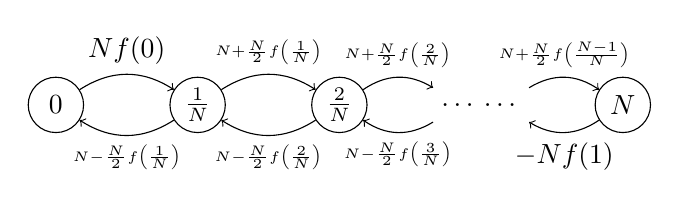
\begin{tikzpicture}[xscale=.9]
    \foreach \x/\y in {0/0, 1/$\frac{1}{N}$, 2/$\frac{2}{N}$, 4/$N$} {%
      \node[draw,circle,inner sep=0pt,minimum size=20] at (2*\x,0) (\x) {\y};%
    };%
    \node[minimum size=12] at (5.7,0) (dots1) {$\dots$};%
    \node[minimum size=12] at (6.3,0) (dots2) {$\dots$};%
    \draw[->] (0) edge[bend left] node[above]{$Nf(0)$} (1);%
    \draw[->] (1) edge[bend left] node[above]{\tiny$N{+}\frac{N}2f\Big(\frac{1}{N}\Big)$} (2);%
    \draw[->] (2) edge[bend left] node[above]{\tiny$N{+}\frac{N}2f\Big(\frac{2}{N}\Big)$}(dots1);%
    \draw[->] (dots2) edge[bend left] node[above]{\tiny$N{+}\frac{N}2f\Big(\frac{N-1}{N}\Big)$} (4);%
    \draw[->] (4) edge[bend left] node[below]{$-Nf(1)$}  (dots2);%
    \draw[->] (dots1) edge[bend left] node[below]{\tiny$N{-}\frac{N}2f\Big(\frac{3}{N}\Big)$}  (2);%
    \draw[->] (2) edge[bend left] node[below]{\tiny$N{-}\frac{N}2f\Big(\frac{2}{N}\Big)$}  (1);%
    \draw[->] (1) edge[bend left] node[below]{\tiny$N{-}\frac{N}2f\Big(\frac{1}{N}\Big)$}  (0);%
  \end{tikzpicture}
  \caption{Transition graph of the birth-death example. }
  \label{fig:BD_graph}
\end{figure}

It should be clear that this process is a population process with
drift $f$.  For $\alpha=0$, $f$ is Lipschitz-continuous and not
differentiable. For $\alpha=1$, $f$ is differentiable and its
derivative is Lipschitz-continuous. For $\alpha\in(0,1)$, the drift is
differentiable and its derivative is $\alpha$-Hölder
continuous. 
In the remainder of this section, we study how $\alpha$ affects the
convergence rate of $\sesp{\XN}-x$ and of $\sesp{\snorm{\XN-x}}$.


\subsection{Differentiability of the Drift}
\label{sec:BD}

When $f$ is Lipschitz-continuous, $\sesp{\snorm{\XN-x}}$ converges at
rate $O(1/\sqrt{N})$ as $N$ goes to infinity
\cite{benaim2008class,kurtz70}. In general, the $O(1/\sqrt{N})$ is
tight: It is the rate of convergence of the central limit theorem. We
verify this in Figure~\ref{fig:rate_fL-f2}(a) where we plot
$\sesp{|\XN(1)-x(1)|}$ as a function of $N$ with an initial state of
$\XN(0)=0.5$. We observe that it decreases as $O(1/\sqrt{N})$, (the
axes are in log-scale). We also display a curve $c/\sqrt{N}$.

\begin{figure}[ht]
  \centering
  \begin{tabular}{@{}c@{}c@{}}
    \includegraphics[width=.5\linewidth]{rate_birthRate_norm2}
    &\includegraphics[width=.5\linewidth]{rate_birthRate}\\
    (a) $\sesp{\snorm{\XN(1)-x(1)}}$ & (b) $|\sesp{\XN(1)}-x(1)|$
  \end{tabular}
  \caption{Convergence rate in the case of the birth-death
    example. The Hölder exponent $\alpha$ has no impact on the rate of
    convergence of $\sesp{|\XN-x|}$ but does affect the rate of
    convergence of $|\sesp{\XN}-x|$.}
  \label{fig:rate_fL-f2}
\end{figure}

The situation of $\sesp{\XN}-x$ is
different. Theorems~\ref{th:transient} and \ref{th:Holder} show that
the convergence rate is at least $O(1/\sqrt{N}^{1+\alpha})$.  In
Figure~\ref{fig:rate_fL-f2}(b), we plot as a function of $N$ the
difference $|\sesp{\XN}-x|$ for $\alpha\in\{0,0.5,1\}$.  We also plot
the function $cN^{-e}$ that best fits the curve. In each case, the
best fit value of the exponent is exactly $(1+\alpha)/2$.  This figure
indicates that the exponent provided in Theorem~\ref{th:Holder} cannot
be improved.

An important observation is that the Lipschitz-continuity of the drift
is not sufficient to obtain an $O(1/N)$ convergence.  This example
shows that mean-field approximation is more accurate when the drift is
not only Lipschitz-continuous but also has a derivative that is
Lipschitz-continuous. 



\subsection{Influence of the Hölder Exponent}


In Figure~\ref{fig:expo_BD}, we study in more detail the impact of the
exponent $\alpha$ on the rate of convergence in transient and
stationary regime. In both cases, we observe that the exponent
$(1+\alpha)/2$ given by Theorem~\ref{th:Holder} cannot be improved.

We used a numerical procedure to compute the values of
$\sesp{|\XN(t)-x(t)|}$ and of $|\sesp{\XN(t)}-x(t)|$ for
$\alpha\in[0,1]$. The value for $t=1$ is computed by integrating the
Kolmogorov equation while the steady-state value is easily obtained
because the process is a birth-death process. In all tested cases, we
observed a convergence in $cN^{-e}$. In Figure~\ref{fig:expo_BD}, we
report an estimation of the value of this exponent $e$ as a function
$\alpha$.  This figure confirms that the exponent of
Theorem~\ref{th:Holder} is tight: For this model, the convergence
occurs at rate $O(1/\sqrt{N}^{1+\alpha})$.  Also, for this model, the
exponent of the rate of convergence of the stationary distribution is
the same as the one for the transient regime.  Note again that the
Hölder coefficient of the drift's derivative has no impact on the
convergence rate of $\sesp{\snorm{\XN-x}}$, neither in the transient
nor in the stationary regime.

\begin{figure}[ht]
  \centering
  \includegraphics[width=0.90\linewidth]{exponent_birthDeath}
  \caption{Estimation of the exponent of the rate of convergence
    $O(N^{-\beta})$. For a drift that has a derivative that is
    $\alpha$-Hölder continuous, this exponent is $(1+\alpha)/2$ for
    $\sesp{\XN}-x$ and is $1/2$ for $\sesp{\snorm{\XN-x}}$.}
  \label{fig:expo_BD}
\end{figure}


\section{Application : Two-Choice Model}
\label{sec:two-choice}

The two-choice paradigm is a well studied model since
\cite{mitzenmacher1996power,vvedenskaya1996queueing}. In this section,
we show that this model satisfies the assumptions of
Theorems~\ref{th:transient} and \ref{th:stationary}. We use these
theorems to show that the marginal law and the average queue length in
steady-state converge at rate $O(1/N)$ to their mean-field
approximation. We also evaluate the constant of the $O(1/N)$
numerically and provide numerical evidence that it evolves as
$1/(2-2\rho)$ as the load of the system $\rho$ goes to $1$. By using
this, we develop an improved approximation that is
$O(1/N^2)$-accurate.


\subsection{Two-choice Model}
\label{sec:two-choice-model}

We consider the supermarket model of \cite{mitzenmacher1996power} with
$N$ identical servers. Each server maintains a separate queue. Jobs
arrive in the system according to a Poisson process with intensity
$N\rho$ and the processing time of a job is exponentially distributed
with mean $1$. We denote by $\SN_n(t)$ the queue size of the server
$n$ at time $t$. For each incoming job, two queues (say $i$ and $j$)
are selected uniformly at random and the job is allocated to the
smallest queue among those two. Note that for all $N$,
$(\SN_1(t)\dots \SN_N(t))$ is a CTMC and has a unique stationary
distribution when $\rho<1$.

Let $\XN_i(t)$ denotes the fraction of servers that have a queue size
at least $i$ at time $t$. Let $\mathbf{e}_i$ denote the infinite
vector where the $i$th component equals $1$, all others being equal to
$0$.  $\XN$ is a CTMC with the following transitions (for all
$i\ge1$):
\begin{itemize}
\item $X \mapsto X-\frac{1}{N}\mathbf{e}_i$ at rate $N(X_{i}-X_{i+1})$;
\item $X \mapsto X+\frac1N\mathbf{e}_i$ at rate
  $N\rho(X^2_{i-1}-X^2_{i})$.
\end{itemize}
The first type of events correspond to a departure from a queue with
$i$ jobs. The second term corresponds to an arrival at a queue with
$i-1$ jobs : An arrival is allocated to a queue with $i-1$ jobs if
both queues have at least $i-1$ jobs and not both queues have $i$ or
more jobs.

The form of these transitions indicates that $\XN$ is a population
process, as defined in Section~\ref{sec:model}. The corresponding
mean-field approximation of this system is given by the following
infinite system of ODEs:
\begin{align*}
  \dot{x}_i &= \rho(x^2_{i-1}-x_i^2) + x_{i+1}-x_{i}
  &\text{for $i\ge1$}\\
  x_0 &= 1.
\end{align*}
It is shown in \cite{mitzenmacher1996power} that this ODE converges
exponentially fast to its unique fixed point
$\pi=(\pi_0,\pi_1,\dots)$, where
\begin{align*}
  \pi_{i} = \rho^{2^i-1}.  
\end{align*}
This guarantees that the stationary distribution of $\XN$ concentrates
on $\pi$ as $N$ goes to infinity.  In the following, we analyze the
rate at which this concentration occurs. 


\subsection{Rate of Convergence} 

The only difficulty for applying the results of
Section~\ref{sec:convergence} is that the queue sizes are unbounded
and that therefore, $\XN$ lives in an infinite-dimensional space. In
the following, we equip the space of infinite sequences with a
weighted $\ell_1$-norm with a carefully chosen sequence $w$. We denote
the norm of an infinite sequence $x$ by $\norm{x}_w$:
\begin{align*}
  \norm{x}_w=\sum_{i=1}^\infty w_i\abs{x_i}.
\end{align*}
Let $\E$ be the set of sequences $x$ such that $\norm{x}_w<\infty$.
The process $\XN$ lives in a subset of $\E$ for each $N$: Indeed, the
sequence $(\XN_i)_i$ is non-negative, non-increasing, and as there is
a finite number of jobs in each server, there is only a finite number
of indices $i$ for which $\XN_i>0$. Such a sequence satisfies
$\snorm{\XN}_w<\infty$ and is therefore in $\E$.

The next result, whose proof is given in Section~\ref{sec:proof_2c},
shows that there exists a sequence of weights $w$ such that the model
satisfies the assumptions of
Theorem~\ref{th:stationary}. 
\begin{theorem}
  \label{th:two-choice}
  There exists an increasing sequence of weights $(w_i)_{i\ge0}$ and a
  constant $B$ such that the two-choice model satisfies the
  assumptions of Theorem~\ref{th:stationary} and such that in
  steady-state:
  \begin{align}
    \label{eq:bound_2c}
    \espN{\norm{\XN}_w\mathbf{1}_{\norm{\XN}_w\ge B}}=o\p{\frac1{N}}.
  \end{align}
\end{theorem}

Theorem~\ref{th:stationary} implies that if $h$ is a bounded function,
then the quantity $\sespN{h(\XN)}$ converges to $h(\pi)$ at rate
$O(1/N)$. This is the case for the marginal law of one server by using
the function $h(x)=x_i$ which is bounded by $1$. This shows:
\begin{align*}
  \Proba{\text{a server has $i$ or more jobs}} = \rho^{2^i-1} +
  O\p{\frac1N}. 
\end{align*}
This result sharpens the result of \cite{luczak2007asymptotic} in
which a convergence rate of $O(\log N/N)$ was obtained. 

Equation~\eqref{eq:bound_2c} implies that for any $h$ that grows at
most linearly, $\sespN{h(\XN)}$ converges to $h(\pi)$ at rate
$O(1/N)$.
\begin{coro}
  \label{coro:two-choice}
  Let $h:\E\to\R$ be a twice-differentiable function. Assume that
  there exists constants $a,b$ such that for all $x\in\E$:
  $|h(x)|\le a+b\norm{x}_w$ for the sequence $w$ defined in
  Theorem~\ref{th:two-choice}. Then the stationary measure of the
  $N$-server two-choice model satisfies
  \begin{align*}
    \abs{\espN{h(\XN)}-h(\pi)}=O\p{\frac1N}.
  \end{align*}
\end{coro}
For a vector $X\in\E$, the quantity
$N\sum_{i\ge 1}X_i$ is the total number of jobs in the $N$ servers of
the model. As the weight sequence $w$ is increasing, the function
$h(x)=\sum_ix_i$ satisfies $h(x)=\sum_ix_i\le \norm{x}_w/w_1$. As a
result, the expected number of jobs satisfies
\begin{align}
  \label{eq:avg_2c}
  \espN{\sum_{i\ge1}\XN_i} 
  = \sum_{i\ge1} \rho^{2^i-1} +
  O\p{\frac1N}.
\end{align}
Our result can also be used to bound the mean-square deviation by
using $h(x)=\sum_{i=0}^\infty(x_i-\pi_i)^2$. As $x_i\le1$, this
function is sub-linear:
$h(x)\le \sum_ix_i+\pi_i \le (\norm{\pi}_w + \norm{x}_w)/w_1$. This
shows that for the two-choice model:
\begin{align*}
  \espN{\sum_{i\ge1}(\XN_i-\pi_i)^2} = O\p{\frac1N}. 
\end{align*}
This last result improves the bound of \cite{ying2016twochoice}, in
which a convergence rate of $O((\log N)^3(\log\log N)^6 /N)$ is
obtained. The factor $(\log N)^3(\log\log N)^6$ of
\cite{ying2016twochoice} comes from the fact that the author studies a
truncated finite-dimensional model in order to study the original
model.  This factor is then a bound on the error between the finite
and infinite models.  One advantage of our approach is that we treat
directly the infinite-dimensional system.


To work in the infinite-dimensional case, the main technical
difficulty for applying our approach is to show that
$\sProba{\snorm{\XN}\ge B}=O(1/N^2)$. In our proof of
Theorem~\ref{th:two-choice}, we prove it by using a coupling to bound
the process by a system of $N$ independent $M/M/1$ queues. We then
show in Lemma~\ref{lem:concentration} that the sum of $N$ independent
variables have a third moment and therefore concentrate on a bounded
set at rate $O(1/N^2)$.  


\subsection{Numerical Evaluation}

In this section, we evaluate numerically the $O(1/N)$ of
\eqref{eq:avg_2c}. We provide numerical experiments that show that
when $\rho$ is close to $1$, the difference between the average queue
length of the $N$-server model and the mean-field approximation is
approximately $\rho^2/(2N(1-\rho))$.

\subsubsection{Methodology}

In order to evaluate the term $O(1/N)$, we use a stochastic
simulator\footnote{The code of our simulator and of all scripts needed
  to plot the graphs are available at \githublink.} of the two-choice
model. Our simulator follows strictly the stochastic model that we
described in Section~\ref{sec:two-choice-model}.

To sample from the stationary distribution, we use a starting period
of $10^4N$ events starting from an empty system. We then draw one
sample of a performance indicator by computing an average over the
next $10^6$ events. This gives us one sample. To guarantee confidence
intervals of order $1/N$, the reported results are averages over
$K(N)=\max(500,N^2/100)$ samples. The error bars that are shown on the
figures correspond to the standard confidence intervals for the mean
(\emph{i.e.} $\pm2\sigma/\sqrt{K(N)}$, where $\sigma^2$ is the
empirical variance of our $K(N)$ samples).  The time to simulate
$K(N)$ samples grows as $N^2$: from $10$ seconds for $N=100$ to more
than $1$ hour for $N=1000$.



\begin{figure}[t]
  \centering
  \begin{tabular}{@{}c@{}}
    \includegraphics[width=0.90\linewidth]{2choice_convergence_rho90}\\
  \end{tabular}
  \caption{Two-choice model: convergence of the marginal law of one
    server. We plot $N(p^N_i-\pi_i)$ as a function of $N$ for various
    values of $i$ and $\rho=0.9$. }
  \label{fig:2-choice_x}
\end{figure}

\subsubsection{Marginal law of one server}

We first study the convergence of the marginal distribution of one
object to $\pi$. For the system of size $N$, we denote by $p^N_i$ the
probability that a server has $i$ or more jobs. As the servers are
symmetric, $p^N_i$ equals
\begin{align*}
  p^N_i=\Proba{\SN_1\ge i} = \espN{\XN_i}. 
\end{align*}

By Theorem~\ref{th:two-choice}, the difference between $p^N_i$ and
$\pi_i$ is of order $O(1/N)$. In Figure~\ref{fig:2-choice_x}, we
display the quantity $N(p^N_i-\pi_i)$ as a function of $N$. We report
the values for $\rho=0.9$ and $i\in\{2,3,4,5\}$. The quantity
$N(p^N_i-\pi_i)$ converges rapidly to a constant value.

We also performed simulations for other values of $\rho\in[0.5,0.99]$
for which we observe similar behavior.  This suggests that for each
$\rho\in[0,1)$ and $i\ge1$ there exists a constant $c_{i,\rho}$ such
that
\begin{align}
  \label{eq:c_i_rho}
  p^N_i&=\pi_i + \frac1N c_{i,\rho} + o\p{\frac1N}.
\end{align}


\subsubsection{Average queue length}


We now focus our attention on the average queue length (in
steady-state). We denote by $m^N(\rho)$ the average queue length in
the system of size $N$ and by $m^\infty(\rho)= \sum_{i\ge1}\pi_i$ its
mean-field approximation.

By Corollary~\ref{coro:two-choice},
$m^N(\rho) = m^\infty(\rho)+O(1/N)$. Equation~\eqref{eq:c_i_rho}
suggests that there exists a constant
$d(\rho)=\sum_{i\ge1}c_{i,\rho}$ such that
\begin{align}
  \label{eq:improved_mf}
  m^N(\rho)=m^\infty(\rho) + \frac{1}{N}d(\rho) + o\p{\frac1N}.
\end{align} 
We verify this numerically in Figure~\ref{fig:2-choice_mean}, where we
display $N(m^N(\rho)-m^\infty(\rho))$ as a function of $N$ for various
values of $\rho$.  We observe that in each case, this value stabilizes
quickly. This stabilization is slower as $\rho$ approaches $1$.

\begin{figure}[t]
  \centering
  \includegraphics[width=0.90\linewidth]{2choice_convergence_mean_noLog}
  \caption{Two-choice model: convergence of the average queue length
    $m^N$. We plot $N(m^N-m^{\infty})$ as a function of $N$ for
    various values of $\rho$.  }
  \label{fig:2-choice_mean}
\end{figure}


Equation~\eqref{eq:improved_mf} shows that it is possible to obtain a
more precise approximation by considering the mean-field approximation
plus the $d(\rho)/N$ term. In Table~\ref{tab:2}, we study the accuracy
of this improved approximation in the case $\rho=0.9$. This table
should be compared with Table~\ref{tab:power2} (shown in the
introduction) that shows that the mean-field approximation is
$1/N$-accurate. The improved approximation is indeed much closer to
the value obtained by simulation: We observe that the error of the
improved approximation, $m^N(\rho)-m^{\infty}(\rho)-d(\rho)/N$,
diminishes at rate $O(1/N^2)$.  The $O(1/N^2)$ error term that we
observe in Table~\ref{tab:2} is the next term in the asymptotic
expansion of $m^N(\rho)$, after the first term in $d(\rho)/N$.


\begin{table}[t]
  \centering
  \begin{tabular}{@{}|@{}c@{}|c|c|c|c|c|}
    \hline
    $N$
    &$  10$  &$  20$  &$  30$  &$  50$ & $+\infty$  \\\hline $m^N(\rho)$
    &$2.804$ &$2.566$ &$2.491$ &$2.434$&-- \\\hline $m^\infty(\rho){+}d(\rho)/N$ 
    &$2.759$ &$2.556$ &$2.488$ &$2.434$&$2.353$ \\\hline Error
    &$4. 10^{-2}$&$1 . 10^{-2}$&$2 .10^{-3}$&$3 . 10^{-4}$&--\\
    \hline
  \end{tabular}
  \caption{Average queue length in the two-choice model (for
    $\rho=0.9$). The values for a finite number of servers  $N$ are obtained by
    simulation. The error is the distance between $m^N$ and the
    corrected mean-field approximation $m^\infty(\rho)+d(\rho)/N$. It is
    proportional to $1/N^2$.}
  \label{tab:2}
\end{table}



\paragraph*{Evolution of $d(\rho)$}
As observed in Figure~\ref{fig:2-choice_mean}, the constant $d(\rho)$
increases rapidly as $\rho$ approaches $1$.  To evaluate how $d(\rho)$
evolves with $\rho$, we plot in Figure~\ref{fig:C_rho}(a) an estimate
of the quantity $d(\rho)$ as a function of $\rho$. Our estimate of
$d(\rho)$ is the experimental value for $N=1000$,
$1000(m^{1000}(\rho)-m^\infty(\rho))$.  We also plot the function
$\rho^2/(2-2\rho)$.  We observe that this function fits very well the
values for $\rho\in[0.5;0.99]$. To confirm this, we also plot
$d(\rho)(1-\rho)/\rho^2$ as a function of $\rho$ in
Figure~\ref{fig:C_rho}(b). This figure suggests that it converges to
$1/2$ as $\rho$ goes to $1$.

The average queue length of the mean-field limit has been shown in
\cite{mitzenmacher1996power} to be of order $\log (1/(1-\rho))$ as
$\rho$ tends to $1$: more precisely,
$\lim_{\rho\to1}m^\infty(\rho) / \log(1/(1-\rho)) = 1/\log2$.  This is
an order of magnitude smaller than when jobs are allocated at random
in which case the average queue length is $1/(1-\rho)$. Our numerical
result suggests that for a finite system size $N$, a term in
$O(1/(N(1-\rho)))$ remains.

We conjecture that the average queue length of a $N$-server two-choice
system satisfies 
\begin{align*}
  m^N(\rho) = \Theta_{\rho\to1}\Big(\log\frac1{1-\rho}\Big)
  + \frac{1}{N}\Theta_{\rho\to1}\Big(\frac{1}{1-\rho}\Big) +
  O\p{\frac1{N^2}}. 
\end{align*}
with a hidden constant of $1/2$ in the term
$\Theta_{\rho\to1}(1/(1-\rho))$. This term is equal to $d(\rho)$ and
seems to satisfy
\begin{align*}
  \lim_{\rho\to1}  (1-\rho) d(\rho)  = \frac12.
\end{align*}


\begin{figure}[ht]
  \centering
  \begin{tabular}[ht]{@{}c@{}c@{}}
    (a)&\begin{tabular}{@{}c}\includegraphics[width=.93\linewidth]{jsq2_simulate/C_rho}
        \end{tabular}\\
    (b)&\begin{tabular}{@{}c}\includegraphics[width=.93\linewidth]{jsq2_simulate/C_rho_conv}
        \end{tabular}
  \end{tabular}
  \caption{Evaluation of $d(\rho)$ as a function of $\rho$. In (a), we
    plot the two curves $d(\rho)$ and $\rho^2/(2-2\rho)$ that are
    almost indistinguishable. In (b), we plot $d(\rho)(1-\rho)/\rho^2$
    which seems to go to $1/2$ as $\rho$ goes to $1$.  }
  \label{fig:C_rho}
\end{figure}



%\newpage
\section{Proofs}
\label{sec:proofs}

\subsection*{Notations} 
For a function $f:\E\to\F$ and $g:\F\to\mathcal{G}$, we denote by
$Df(x)$ the derivative of the function $f$ evaluated at $x$. $Df(x)$
is a linear map that associates to each $u$ the quantity
$Df(x)\cdot u$.  We denote by $D(f(g(x)))$ the derivative of the
function $f\circ g$ with respect to $x$ evaluated at $x$ and by
$Df(g(x))$ the derivative of $f$ evaluated at $g(x)$. It follows
that $D(f(g(x)))=Df(g(x))\cdot
Dg(x)$.  

We define the following operators $\PsiN_t$ and $\Phi_t$ that operate
on $h:\E\to\R$:
\begin{align}
  \PsiN_t h (x) &= \esp{ h(\XN(t)) \mid \XN(0) = x} \label{eq:operatorN}\\
  \Phi_t h (x) &= h( \Phi_tx ) \label{eq:operatorInf}
\end{align}
For a function $h\in C^1(\E,\R)$, we have
$\dt \PsiN_th = \PsiN_t\LN h= \LN\PsiN_t h$ and
$\dt \Phi_th = \Phi_t\Lambda h= \Lambda\Phi_t h$.




\subsection{Proof of Theorem~\ref{th:transient} (Transient Regime)}
\label{sec:proof_t}

The proofs of the following lemmas follow similar ideas as the proof
of \cite[Theorem~1]{kolokoltsov2011mean}. Yet, we provide a complete
proof here as our result generalizes
\cite[Theorem~1]{kolokoltsov2011mean} for two reasons.  First, the set
of transitions that we consider is more general (a transition in the
model of \cite{kolokoltsov2011mean} can only affect one
object). Second, our results apply for Banach space and not just for
finite dimensional sets.

\begin{lemma}
  \label{lem:trotter-kurtz}
  For any $h\in C^{1}(\E,\R)$, we have
  \begin{align}
    \esp{\abs{h(\XN(t))-h(\Phi_tx)}} \le
    \int_0^t\!\sup_{x\in\E}|(\Lambda-\LN)h(\Phi_sx)|ds.
    \label{eq:lem_TK}
  \end{align}
\end{lemma}
\begin{proof}
  By definition of the operators $\PsiN$ and $\Phi$ introduced in
  \eqref{eq:operatorN} and \eqref{eq:operatorInf}, the left-hand side
  of Equation~\eqref{eq:lem_TK} can be written as
  \begin{align*}
    \esp{h(\XN(t))-h(\Phi_tx)} = \PsiN_thx-\Phi_thx =
    (\PsiN_t-\Phi_t)hx. 
  \end{align*}
  We are therefore interested in the convergence of
  $\PsiN_t-\Phi_t$. 

  As in \cite[Theorem~1]{kolokoltsov2011mean}, we use the following
  trick : The function $s\mapsto\PsiN_{t-s}\Phi_s$ is equal to
  $\Phi_t$ for $s=t$ and $\PsiN_t$ for $s=0$.  Hence:
  \begin{align}
    \Phi_t - \PsiN_t  &= \int_0^t \frac{d}{ds} \PsiN_{t-s}\Phi_s ds\nonumber\\
                       &=\int_0^t \PsiN_{t-s}(\Lambda-\LN)\Phi_sds. 
                         %\label{eq:Poisson_transient}
  \end{align}
  For any function $h'$, one has
  \begin{align*}
    \abs{\PsiN_{t-s}h'x} &= \abs{\espN{h'(\XN(t-s))\mid \XN(0)=x}}
                         \le\sup_{x\in\E} \abs{h'(x)}. 
  \end{align*}
  This shows that for any $h$ and any $x$: 
  \begin{align*}
    \abs{\PsiN_thx -  \Phi_thx} \le \int_0^t\sup_{x\in\E}
    \abs{(\Lambda-\LN)\Phi_shx}ds,
  \end{align*}
  which is Equation~\eqref{eq:lem_TK}. 
  \end{proof}


\textbf{Remark}: \emph{ Although Theorem~\ref{th:transient} is stated
  only in the Lipschitz-continuous case, the proof in this section
  holds for $\alpha$-Hölder continuous. This does not require more
  work and will be useful for the proof of
  Equation~\eqref{eq:Holder_ss}.}

\begin{lemma}
  \label{lem:Holder}
  Assume that $Df$ is bounded and is $\alpha-$Hölder continuous with
  constant $L$. Then, there exists a constant $\beta$ such that, for
  any $t$, $\Phi_t$ is $\alpha$-Hölder continuous with constant
  $Le^{\beta t}$.
\end{lemma}
\begin{proof}
  Let $x,e\in\E$. By \cite[Theorem~3.7.1 of Part~II]{cartan1977cours},
  $D\Phi_t(x)$ and $D\Phi_t(x+e)$ exist and are differentiable with
  respect to time. Moreover,
  $\dt D\Phi_t=D(f(\Phi_t))=Df(\Phi_t)\cdot D\Phi_t(x)$. As
  $\norm{D\Phi_0}=1$, this shows $\norm{D\Phi_t}\le\exp(t\norm{Df})$.

  Let $F_t=D\Phi_t(x+e)-D\Phi_t(x)$. We have
  \begin{align}
    \dt F_t &= \dt \p{D\Phi_t(x+e)-D\Phi_t(x)}\nonumber\\
            &= D(f(\Phi_t(x+e))) - D(f(\Phi_t))\nonumber\\
            &= Df (\Phi_t(x+e))\cdot D\Phi_t(x+e) - Df(\Phi_tx)\cdot
              D\Phi_t(x)\nonumber\\
            &= Df (\Phi_t(x+e))\cdot F_t \nonumber\\
            &\qquad -\p{Df(\Phi_t(x+e))-Df(\Phi_tx)}\cdot D\Phi_t(x)
              \label{eq:dF_t}
  \end{align}
  
  By using the Hölder-continuity of $Df$ and the fact that
  $\norm{D\Phi_t}\le e^{t\norm{Df}}$, the second term of
  Equation~\eqref{eq:dF_t} is bounded by
  \begin{align*}
    \norm{Df(\Phi_t(x+e))-Df(\Phi_tx)}
    &\le L\norm{D\Phi_t(x+e)-Df(\Phi_tx)}^\alpha\\
    &\le L(e^{t\norm{Df}}\norm{e})^\alpha 
  \end{align*}

  The quantity $\norm{F_t}$ can then be bounded by using Gronwall's
  Lemma:
  \begin{align*}
    \norm{F_t}&\le \int_0^t(\norm{Df} \norm{F_s} +
    L(e^{t\norm{Df}}\norm{e})^\alpha)ds \\
              &\le L e^{t(1+\alpha)\norm{Df}}\norm{e}^\alpha.
  \end{align*}
  The result follows by setting $\beta=(1+\alpha)\norm{Df}$.
\end{proof}



\subsection{Proof of Theorem~\ref{th:stationary} and of
  Equation~\eqref{eq:Holder_ss} (Stationary Regime)}
\label{sec:proof_ss}

\textbf{Remark}: \emph{As for Lemma~\ref{lem:Holder}, we directly
  prove the result in the case of $\alpha$-Hölder continuous
  derivative.  Theorem~\ref{th:stationary} can be obtained by
  considering the special case $\alpha=1$. } \medskip

\begin{lemma}
  \label{lem:proof_ss} 
  Let $\Phi_t$ be the flow associated to a drift $f:\E\to\E$ that is
  differentiable with a bounded derivative. Let $\calB\subset\E$ be a
  bounded set. Assume that $f$ is $\alpha$-Hölder continuous and that
  the flow has an exponentially stable attractor $x^*$.
  \begin{itemize}
  \item[(i)] There exists $b,\delta>0$ such that for any $t$:
    \begin{align*}
      \sup_{x\in\calB}\norm{D\Phi_t}\le be^{-\delta t}. 
    \end{align*}
  \item[(ii)] There exists a constant $c$ such that, the derivative of
    $x\mapsto\Phi_tx$ exists and is $\alpha$-Hölder continuous on
    $\calB$ with constant $ce^{-\delta t}$.
  \item[(iii)] The function $Gh$, defined by 
    \begin{align*}
      Gh : x\mapsto \int_0^\infty \p{h(\Phi_t x)-h(x^*)}dt, 
    \end{align*}
    is differentiable on $\calB$ and its derivative is $\alpha$-Hölder
    continuous.
  \end{itemize}
\end{lemma}

\begin{proof}
  We will first prove \emph{(i)}, then prove that \emph{(i)} implies
  \emph{(ii)} and then prove \emph{(iii)}.  The most technical part of
  our proof is to show that \emph{(i)} implies \emph{(ii)}. Its proof
  is inspired by the proof of \cite[Lemma~C.1]{eldering2013normally}
  that shows that the exponential decay of the first derivative of
  the flow implies the exponential decay of the second derivative of a
  flow.
  
  \textbf{Proof of \emph{(i)}} -- To ease the notation, we assume
  without loss of generality that $x^*=0$. By assumption, $0$ is
  exponentially stable, which means that there exists $\beta>0$ such
  that $\norm{\Phi_t(x)}\le e^{-\beta t}\norm{x}$.

  Let $A=Df(0)$.  As $Df$ is continuous at $x^*=0$, $f(x)=Ax + g(x)$
  and $Df(x)=A+h(x)$ where the functions $g$ and $h$ satisfy
  $\lim_{x\to0}\norm{g(x)}/\norm{x}=0$ and
  $\lim_{x\to0}\norm{h(x)}=0$. Let $\delta=\beta/2$. By assumption,
  there exists a neighborhood $\calN$ of $0$ such that
  $\norm{g(x)}\le\delta\norm{x}$ and $\norm{h(x)}\le\delta$ for
  $x\in\calN$. As the flow is stable, there exists a neighborhood
  $\calN'$ of $0$ such that if $x\in\calN'$, then $\Phi_tx\in \calN$
  for all $t\ge0$.
  
  The flow satisfies
  \begin{align*}
    \Phi_tx &= e^{At}x + \int_0^t e^{A(t-s)} g(\Phi_sx)ds
  \end{align*}
  As the flow is exponentially stable, it is also linearly stable:
  $\norm{e^{At}}\le e^{-\beta t}$. Hence, for all $x,x+y\in\calN'$:
  \begin{align*}
    & \norm{\Phi_t(x+y) - \Phi_tx}\\
    &= \norm{e^{At}y + \int_0^t e^{A(t-s)}
      (g(\Phi_s(x+y))-g(\Phi_sx))ds}\\
    &\le e^{-\beta t}\norm{y} \\
    &\qquad+ \int_0^t
      e^{-\beta(t-s)} \underbrace{\sup_{x\in 
      N_\varepsilon}\norm{h(x)}}_{\le\delta}\norm{\Phi_s(x+y)-\Phi_s(x)}ds. 
  \end{align*}
  Therefore, $z(t)=\norm{\Phi_t(x+y)-\Phi_tx}e^{\beta t}$ satisfies
  \begin{align*}
    z(t)\le \norm{y} + \delta \int_0^t z(s)ds \le
    \sup_{y\in\calN'}\norm{y}e^{\delta t}
  \end{align*}
  This shows that $\Phi_t$ is Lipschitz-continuous on $\calN'$ with a
  constant less than $ae^{-\delta t}$ with
  $a=\sup_{y\in\calN'}\norm{y}$. By Lemma~\ref{lem:Holder}, $D\Phi_t$
  is continuous, which implies that
  $\norm{D\Phi_t}\le ae^{-\delta t}$. 
  
  The set $\calB$ is a bounded subset of $\E$ and $0$ is exponentially
  stable. Hence, there exists $T$ such that for all $x\in\calB$, we
  have $\Phi_t(x)\in \calN'$.  Let $x\in\calB$. For $t\ge T$, we have
  \begin{align*}
    \norm{D\Phi_tx} &= \norm{ D(\Phi_{t-T}\circ\Phi_{T})}
    =\norm{ D\Phi_{t-T}(\Phi_{T}) \cdot D\Phi_{T}}\\
                    &\le a^{-\delta(t-T)}e^{\norm{Df}T}
    \le b e^{-\delta t},
  \end{align*}
  with $b=a^{\delta T + \norm{Df}T}$.
  
  \textbf{Proof of (i)$\Rightarrow$\emph{(ii)}} -- As in the proof of
  Lemma~\ref{lem:Holder}, let $F_t=D\Phi_t(x+e)-D\Phi_t(x)$.
  Following, Equation~\eqref{eq:dF_t}, $F_t$ satisfies the
  differential equation
  \begin{align}
    \dt F_t &= Df (\Phi_t(x+e))\cdot F_t \nonumber\\
            &\qquad -\p{Df(\Phi_t(x+e))-Df(\Phi_tx)}\cdot D\Phi_t(x)
              \label{eq:nonHomoODE}
  \end{align}
  with initial condition $F_0=D(\Phi_0(x+e))-D\Phi_0(x)=0$. 
  
  The homogeneous part of the differential equation is
  $\dot{A} = Df(\Phi_t(x+e)) A$. It is a linear differential equation
  on $\calL(\E,\E)$, the set of linear map from $\E$ to $\E$. Let
  $A_{t,s}:\calL(\E,\E)\to \calL(\E,\E)$ be the solution
  operator\footnote{This means that for $y\in\calL(\E,\E)$, the
    function $s\mapsto A_{t,s}y$ is the solution of the homogeneous
    differential equation starting in $y$ at time $s$.} of this
  homogeneous differential equation.
  
  Let $F:\R^+\to\calL(\E,\E)$ be the function defined by
  \begin{align*}
    F_t = \int_0^t A_{t,s}\p{Df(\Phi_s(x+e))-Df(\Phi_sx)}\cdot
    D\Phi_sxds.
  \end{align*}
  Let us show that $F$ is indeed the function $F$ defined at the
  beginning of the proof by showing that it is a solution of the
  differential equation \eqref{eq:nonHomoODE}. By definition of $F$,
  we have $F_0=0$. Moreover, for $t>0$, we have 
  \begin{align*}
    \dt F_t &= \int_0^t \dt A_{t,s}\p{Df(\Phi_s(x+e))-Df(\Phi_sx)}\cdot 
              D\Phi_s xds \\
            &\qquad +  A_{t,t} \p{Df(\Phi_t(x+e))-Df(\Phi_tx)}\cdot D\Phi_t x\\
            &= Df(\Phi_t(x+e)) \cdot F_t \\
            &\qquad +  \p{Df(\Phi_t(x+e))-Df(\Phi_tx)}\cdot
              D\Phi_tx. 
  \end{align*}
  
  The solution operator $A$ satisfies
  $A_{t,s}\mathbf{1}=D\Phi_{t-s}x$. Hence, by using \emph{(i)} that
  $\norm{D\Phi_t}\le ae^{-\delta t}$, we have
  $\norm{A_{t,s}}\le ae^{-\delta (t-s)}$. This shows that
  \begin{align}
    \norm{F_t}&\le\int_0^t
                \norm{A_{t,s}}\norm{Df(\Phi_s(x+e))-Df(\Phi_s(x))}\norm{D\Phi_sx}ds
                \nonumber\\ 
              &\le \int_0^t ae^{-\delta (t-s)}
                L\norm{\Phi_s(x+e)-\Phi_sx}^\alpha a e^{-\delta s}ds,
                \label{eq:bound_F_t}
  \end{align}
  where $L$ is the Hölder constant of $Df$. 

  By using again \emph{(i)} ($\norm{D\Phi_t}\le ae^{-\delta t}$), we
  have
  \begin{align*}
    \norm{\Phi_s(x+e)-\Phi_sx} \le \norm{\Phi_s}\norm{e} \le
    ae^{-\delta s}\norm{e}
  \end{align*}
  Plugging this bound into Equation~\eqref{eq:bound_F_t} shows
  \begin{align*}
    \norm{F_t}&\le \int_0^t ae^{-\delta (t-s)}
                L(a e^{-\delta s})^\alpha  a e^{-\delta
                s}ds \norm{e}^\alpha \\
              &= L a^{2+\alpha} e^{-\delta t} \int_0^t
                e^{-\delta\alpha s}ds\norm{e}^\alpha\\
              & = L a^{2+\alpha} e^{-\delta t} \frac{1}{\delta \alpha}
                (1-e^{-\delta\alpha t})\norm{e}^\alpha
  \end{align*}
  This shows that $\norm{F_t}\le c e^{-\delta t}\norm{e}^\alpha$ with
  $c:=L a^{2+\alpha}/(\delta\alpha)$.

  % Note that this proof can be adapted to higher order dimension,
  % following the approach of \cite[Lemma~C.1]{eldering2013normally}. In
  % particular, if $f$ and $h$ are $C^k$, then $Gh$ is also $C^k$.

  \textbf{Proof of \emph{(iii)}} -- Lemma~\ref{lem:Holder} shows that
  for all $t$, the derivative of $\Phi_t$ exists and is
  $\alpha$-Hölder continuous. By \emph{(i)}, the derivative of $Gh$
  exists and is equal to 
  \begin{align*}
    D(Gh)= \int_0^\infty D(\Phi_th) dt. 
  \end{align*}
  By \emph{(ii)}, $D(\Phi_th)$ is $\alpha$-Hölder continuous with
  constant $Lce^{-\delta t}$. This shows that the function $D(Gh)$ is
  $\alpha$-Hölder continuous with constant
  $\int_0^\infty Lce^{-\delta t}dt = Lc/\delta$.
\end{proof}

\subsubsection{Dealing with non-compact state-space}

\begin{lemma}\label{lem:proof_ss2} Assume that the system satisfies the
  assumption of Theorem~\ref{th:stationary} and the function $h$
  equals $h(x^*)$ outside a bounded set. Then there exists a constant
  $B'$ such that
  \begin{align*}
    \espN{(\Lambda-\LN)Gh(\XN)\mathbf{1}_{\XN\not\in\calB}}<B'/N.
  \end{align*}
\end{lemma}

\begin{proof}
  Let $W$ be a bounded set outside containing the set $V$ of
  Assumption~(A2) and outside which $h(x)$ is equal to $h(x^*)$. For
  $x\in\E$, let $S(x)$ be the first time at which the solution of the
  ODE that starts in $x$ enters $W$ -- the function $S(x)$ exists
  because $V\subset W$ and $V$ attracts all trajectories. We have
  \begin{align*}
    Gh x &= \int_0^\infty (h(\Phi_t x) - h(x^*)) dt\\
         &=\int_0^{S(x)}\hspace{-.3cm}\underbrace{(h(\Phi_t
           x) - h(x^*))}_{=0}dt + 
           \int_{S(x)}^{\infty}\hspace{-.3cm}(h(\Phi_t x) - h(x^*))dt\\
         &=Gh(\Phi_{S(x)}x).
  \end{align*}
  As $W$ is bounded and $Gh$ is continuous, there exists $v<\infty$
  such that $\sup_{x\in W}\norm{Ghx}\le v<\infty$. Moreover, by
  definition of $S(x)$, we have $\Phi_{S(x)}x\in W$ which implies that
  for all $x$, $\norm{Ghx}\le v$.  This shows that
  \begin{align*}
    (\LN Gh)(x) &= \norm{\sum_{\ell\in\calL}
                  N\beta_\ell(x)\p{(Gh)(x+\frac{\ell}{N})-(Gh)(x)}}\\
                &\le N \sup_{x'\in\E}\sum_{\ell\in\calL}\beta_\ell(x')
                  2v
  \end{align*}
  Let
  $b:=2v\sup_{x'\in\E}\sum_{\ell\in\calL}\beta_\ell(x')+2\sup_{x}\norm{h(x)}<\infty$. By
  using that $\Lambda(Gh)(x)=h(x)-h(x^*)$, we have
  \begin{align*}
    \norm{(\Lambda- \LN)(Gh)(x)} \le bN
  \end{align*}
  This shows that 
  \begin{align*}
    \espN{ (\Lambda-\LN)(Gh)(\XN)\mathbf{1}_{\XN\not\in\calB}}
    \le \espN{Nb},
  \end{align*}
  which is of order $O(1/N)$ by Assumption~(A3).
\end{proof}

\subsection{Proof of Theorem~\ref{th:Holder} (Hölder-continuity)}
\label{sec:Holder_proof}

To simplify the notation, we assume that $\XN(0)=x$.

By \cite{kurtz1978strong}, $\XN$ is equal to
\begin{align*}
  \XN(t) = \XN(0) + \int_0^t f(\XN(s))ds + M_t,
\end{align*}
where $M_t$ is a martingale (in particular $\esp{M_t}=0$) that
satisfies $\esp{\norm{M_t}^2}\le C^2_t/N$ for some constant $C_t>0$.
Let $\YN(t)=\XN(t)-\Phi_tx$. As $\Phi_tx=x + \int_0^tf(\Phi_sx)ds$ and
$\YN(0)=0$, the quantity $\YN$ satisfies
\begin{align}
  \YN(t) =  \int_0^tf(\Phi_sx+\YN(s))-f(\Phi_sx)ds + M_t.
  \label{eq:YN}
\end{align}
Let $H$ be the max between the Lipschitz-constant of $f$ and the
Hölder-constant of $Df$.  By Gronwall's Lemma \cite[Lemma~1.5.1, Part
II]{cartan1977cours}
\begin{align*}
  \esp{\norm{\YN(t)}^2}\le \frac{2C^2_te^{2H^2t}}{N}.
\end{align*}
%where $H$ is the Lipschitz-constant of $f$. 

As $Df$ is $\alpha$-Hölder continuous, for any $x,y\in\E$ we have\\
$\norm{f(x+y)-f(x)- Df(x)\cdot y}\le H\norm{y}^{1+\alpha}$.  As a
result, for a random variable $Y$, we have
\begin{align*}
  \esp{\norm{f(x+Y)-f(x)}}\le \norm{Df}\norm{\esp{Y}} +
  H\esp{\norm{Y}^{1+\alpha}}
\end{align*}
Applying this to Equation~\eqref{eq:YN} shows that
\begin{align*}
  \norm{\esp{\YN(t)}} \le &
  \int_0^t\norm{DF}\norm{\esp{\YN(s)}}ds\\
                   &\qquad+\frac{HT2^{(1+\alpha)/2}e^{H^2t(1+\alpha)}}{N^{(1+\alpha)/2}},
\end{align*}
By Gronwall's lemma \cite[Lemma~1.5.1, Part II]{cartan1977cours}, this
in turns implies the existence of a constant $c$ such that
$\snorm{\sesp{\YN(t)}}\le c e^{ct} N^{-(1+\alpha)/2}$.



\subsection{Proof of Theorem~\ref{th:two-choice} (Two-choice)}
\label{sec:proof_2c}


To prove that the two-choice model satisfies the assumptions of
Theorem~\ref{th:stationary}, the only difficulty is to show that the
fixed point is asymptotically stable (assumptions A1 and A2) and to
show that the stationary measure concentrates on a bounded sub-set of
$\E$ (assumptions A3).  The existence of a sequence of $w$ such that
the two-choice model is asymptotically stable for the weighted
$\ell_1$-norm $\norm{x}=\sum_i w_i x_i$ has been shown in
\cite[Theorem~3.6]{mitzenmacher1996power}. To prove our concentration
result, we also need that this sequence grows slower than
$\rho^{-i/3}$. We construct such a sequence below.

According to \cite[Proof of Theorem~3.6]{mitzenmacher1996power}, the
quantity $V(x)=\norm{x-\pi}_w$ satisfies
$\dt V(\Phi_tx)\le -\delta V(x)$ if the sequence $w_i$ is positive and
satisfies
\begin{equation}
  \label{eq:w_i}
  w_{i+1} \le w_i + \frac{w_i(1-\delta) - w_{i-1}}{\rho
    (2\pi_i+1)},
\end{equation}
where $\pi_i=\rho^{2^i-1}$ is the fixed point of the ODE. 

Let $a=\rho^{-1/4}$ 
and let us show that there exists a sequence
$(w_i)$ and a constant $\delta>0$ that satisfy \eqref{eq:w_i} and such
that $w_i=O(a^i)$.

Let $b\in(a,1/\rho)$. As $b<1/\rho$, there exists $i^*$ such
that $1/(\rho (2\pi_i+1))\ge b$ for $i\ge i^*$. We define a
sequence $w_i$ by $w_0=0$, $w_1=1$ and
\begin{align*}
  w_{i+1} &= w_i+\frac{w_i(1-\delta) - w_{i-1}}{3\rho} 
  &\text{ for $i<i^*$}\\
  w_{i+1} &= aw_i  &\text{for $i\ge i^*$}. 
\end{align*}
By definition of $w$, $w_i=O(a^i$).

As $i^*$ is finite, there exists $\delta^*$ such that for
$\delta\le\delta^*$, the sequence $w_i$ is increasing and satisfies
\eqref{eq:w_i} for $i<i^*$. Let
$\delta=\min(\delta^*,(a-1)(b-a)/(ab))$.  For $i>i^*$, we have
\begin{align*}
  &w_{i+1} - w_i - \frac{w_i(1-\delta)-w_{i-1}}{\rho(2\pi_i+1)} \\
  &\qquad\le w_{i+1}-w_i - b (w_i(1-\delta)-w_{i-1})\\
  &\qquad= a(w_i-w_{i-1}) - b (w_i-w_{i-1}) + \delta b w_{i}\\
  &\qquad= (a-b)(w_i-w_{i-1}) + \delta b w_i \\
  &\qquad= (a-b)\p{1-\frac1a} w_i + \delta b w_i \\
  &\qquad= \p{\frac{(a-b)(a-1)}{a} + \delta b} w_i,
\end{align*}
this shows that $w_i$ satisfies Equation~\eqref{eq:w_i} for
$\delta=\min(\delta^*,(b-a)(a-1)/(ab))>0$.


% Hence, to show (A3) we need to show that there exists a constant $B$
% such that $\sProba{\sum_{i=0}^\infty a^i\XN_i\ge B}=O(1/N^2)$.

According to \cite[Theorem~4]{turner1998effect} (see also
\cite[Theorem~4.1]{graham2000chaoticity}), there exists a coupling
between $\XN$ and a variable $\XtN$ picked according to the
stationary distribution of $N$ independent M/M/1 queues such that for
all $j$, $\sum_{i=j}^\infty\XN_i\le\sum_{i=j}^\infty\XtN_i$. Denoting
$w_0=0$, for any infinite sequence $x$ we have
$\sum_{i=1}^\infty
w_ix_i=\sum_{i=1}^\infty(w_{i}-w_{i-1})\sum_{j=i}^\infty x_j$.
As the sequence $w$ is increasing, $w_i-w_{i-1}\ge0$. This implies
that (for this coupling): 
$\snorm{\XN}_w=\sum_{i=1}^\infty
w_j\XN_j=\sum_{i=1}^\infty(w_{i}-w_{i-1})\sum_{j=i}^\infty\XN_j \le
\sum_{i=1}^\infty(w_i-w_{i-1})\sum_{j=i}^\infty\XtN_j =\norm{\XtN}_w
$.
%is stochastically smaller than $\snorm{\XtN}_w$.

%  A natural
% coupling argument\footnote{Consider the partial order
%   $x\preceq \tilde{x}$ if and only if $x_i\le \tilde{x}_i$ for all
%   $i\ge1$. By coupling the arrivals and departures in a two-choice
%   model $\XN$ and in a one-choice model $\XtN$ (\emph{i.e.} $N$
%   independent M/M/1 queues), the trajectories satisfy
%   $\XN\preceq\XtN$. Hence, there exist a coupling of the variables
%   $\XN$ and $\XtN$ such that $\XN$ and $\XtN$ are always comparable
%   and $\XN\preceq\XtN$.}
% shows that $\XN$ is component-wise bounded
% by a variable $\tilde{\XN}$ that is picked according to the stationary
% distribution of $N$ independent M/M/1 queues. 
In stationary regime, the quantity $\XtN$ can be written as
$\XtN_i=(1/N)\sum_{n=1}^N1_{\tilde{Z}_n\ge i}$ where the variables
$\tilde{Z}_n$ are \emph{i.i.d.} and are geometrically distributed with
parameter $\rho$. The sequence $w$ defined above satisfies
$w_i\le c a^i$. This implies that $\sum_{j=1}^i w_i\le c' a^i$, where
$c'=ca/(a-1)$.  Therefore, in the stationary regime, we have
\begin{align*}
  %\label{eq:XN-le-tilde}
  \norm{\XN}_w\le\norm{\XtN}_w&=\frac{1}{N}\sum_{n=1}^N\sum_{i\ge0} w_i
                                      \mathbf{1}_{\tilde{Z}_n\ge i} 
                     % &\le c' N^-1\sum_{n=1}^N\sum_{i\ge0}
                     % a^i\mathbf{1}_{\tilde{Z}_n=i} \\
  \le \frac{c'}{N}\sum_{n=1}^Na^{\tilde{Z}_n},
\end{align*}
where $c'<\infty$ is the constant defined above.

To conclude, we use the following concentration lemma that we apply
with $\xi_n=a^{\tilde{Z}_n}$. Note that quantity
$\esp{\norm{\xi_n}^3}=\sesp{a^{3\tilde{Z}_n}}$ is finite because
$a<\rho^{-1/3}$ and $\tilde{Z}_n$ is geometrically distributed with
parameter $\rho$.
% Equation~\ref{eq:XN-le-tilde} and Lemma~\ref{lem:concentration}
% imply that
% \begin{align*}
%   \esp{\norm{\XN}_w\mathbf{1}_{\norm{\XN}_w\ge B'}} \le 
%   \esp{\norm{\tilde{\XN}}_w\mathbf{1}_{\norm{\tilde{\XN}}_w\ge B'}}
%   \le \frac{B}{N}. 
% \end{align*}

\begin{lemma}
  \label{lem:concentration}
  Let $(\xi_n)$ be a sequence of \emph{i.i.d.} random variables such
  that $\esp{\norm{\xi_n}^3}<+\infty$. Let
  $S_N=N^{-1}\sum_{n=1}^N\xi_n$. Then there exist two finite constants
  $B$ and $B'$ such that
  $\esp{\norm{S_N}\mathbf{1}_{\norm{S_N}\ge B'}}\le B/N^2$.
\end{lemma}


\begin{proof}%[of Lemma~\ref{lem:concentration}]
  Let $\bar{\xi}_n=\xi_n-\sesp{\xi_n}$ and
  $\bar{S}_N=S_N-\esp{S_N}=S_N-\esp{\xi_1}$. By assumption, there
  exists a constant $B<\infty$ such that
  $\sesp{\snorm{\bar{\xi}_n}^3}\le B$. As the variables $\bar{\xi}_n$
  are \emph{i.i.d}, this implies that
  $\sesp{\snorm{\bar{S}_N}^3}\le B/N^2$. This shows that
  \begin{align*}
    \esp{\norm{\bar{S}_N}\mathbf{1}_{\norm{\bar{S_N}}\ge1}}
    &\le \esp{\norm{\bar{S}_N}^3\mathbf{1}_{\norm{\bar{S_N}}\ge1}}\\
    &\le \esp{\norm{\bar{S}_N}^3}\le
      \frac{B}{N^2}. 
  \end{align*}
  By taking $B'=\esp{\xi_1}+1$, we have
  \begin{align*}
    \esp{\norm{S_N}\mathbf{1}_{\norm{S_N}\ge B'+1}}
    &\le
      B'\proba{\norm{\bar{S}_N}\ge1}+\esp{\norm{\bar{S}_N}\mathbf{1}_{\norm{\bar{S_N}}\ge1}}
    \\
    &\le \frac{B(B'+1)}{N^2}, 
  \end{align*}
  where we use Markov's inequality to show that
  $\proba{\norm{\bar{S}_N}\ge1}=\proba{\norm{\bar{S}_N}^3\ge1^3}\le
  B/N^2$.
\end{proof}

% Let $\alpha=-3/\log\rho=1/(4\log a)$ and let $i_N=\alpha\ln N$.
% According to \cite[Equation~5.3]{vvedenskaya1996queueing},
% $\sesp{\XN_i}\le \rho^i$. Therefore,
% \begin{align*}
%   \espN{\sum_{i=i_N+1}^{\infty} a^i \XN_i}\le
%   \frac{(a\rho)^{i_N}}{1-a\rho}=\frac{n^{\alpha \ln(a\rho)}}{1-a\rho}.
% \end{align*}
% By definition of $\alpha$, $\alpha \ln(a\rho)=-2.75$. This shows that
% $N^{\alpha \ln(a\rho)}=o(N^{-2})$.  Hence, by Markov inequality, we
% have
% \begin{align}
%   \Proba{\sum_{i=i_N+1}^{\infty} a^i \XN_i\ge \frac{1}{1-a\rho}} \le
%   n^{\alpha\ln(a\rho)} = o(N^{-2}). 
%   \label{eq:i_N}
% \end{align}
% According to \cite[Lemma~2.6]{luczak2007asymptotic}, there exists a
% constant $c$ such that 
% % (which can be derived from \cite[Lemma~4.2]{luczak2006maximum}),
% \begin{equation*}
%   \Proba{\sup_{i}\abs{\XN_i-\esp{\XN_i}}\ge cN^{-1/2}\ln N} = o(N^{-2}).
% \end{equation*}
% Summing from $i=0$ to $i_N$ implies that 
% \begin{align*}
%   \Proba{\abs{\sum_{i=0}^{i_N}a^i(\XN_i-\esp{\XN_i})}\ge
%   \sum_{i=0}^{i_N}a^icN^{-1/2}\ln N} = o(N^{-2}). 
% \end{align*}
% As $\sum_{i=0}^{i_N}a^i=(n^{\alpha\ln a}-1)/(a-1)$, we have 
% \begin{align*}
%   \Proba{\sum_{i=0}^{i_N}a^i\XN_i\ge \sum_{i=0}^{i_N}\esp{\XN_i}+
%   cN^{\alpha \ln a-1/2}\ln N} = o(N^{-2}). 
% \end{align*}
% As $\alpha \ln a=1/4\le 1/2$, the quantity
% $cN^{\alpha \ln a-1/2}\ln N$ converges to $0$ as $N$ goes to
% infinity. Moreover, let
% $\sum_{i=0}^{i_N}a^i\sesp{\XN_i}\le 1/(1-a\rho)$. This shows that for
% $N$ large enough, 
% \begin{align}
%   \Proba{\sum_{i=0}^{i_N}a^i\XN_i\ge \frac{1}{1-a\rho}+1} =
%   o(N^{-2}).
%   \label{eq:luczak}  
% \end{align}
% Combining Equation~\eqref{eq:i_N} and \eqref{eq:luczak}  shows that 
% \begin{align*}
%   \Proba{\sum_{i=0}^\infty a^i \XN_i\ge \frac{2}{1-a\rho}+1}
%   =o(N^{-2}).
% \end{align*}
% As $w_i\le c'a^i$, this implies that $\sProba{\snorm{\XN}\ge
%   c'/(1+a\rho)+2}=o(N^{-2})$ which implies (A3). 

% Finally, as
% $\sum_{i=0}^{i_N}a^iX_i^{(N)}\le n^{\alpha\log(a)}/(a-1)=O(N^{1/4})$,
% Equation~\eqref{eq:luczak} shows that
% \begin{align*}
%   \esp{\sum_{i=0}^{i_N}a^i\XN_i\mathbf{1}_{\sum_{i=0}^{i_N}a^i\XN_i\ge
%   \frac{1}{1-a\rho}}} = o(N^{-7/4})=o(N^{-1}) 
% \end{align*}
% As $\esp{\sum_{i=i_N+1}^{\infty}a^i\XN_i}=O(N^{-2.75})$, this implies
% Equation~\eqref{eq:bound_2c}.
% %\newpage
 
\section{Conclusion and discussion}
\label{sec:conclusion}

In this paper, we revisited the rate of convergence of mean-field
models. Most of the results in the literature show that the expected
distance between the empirical measure $\XN$ and its mean-field
approximation $x$ converges to $0$ at rate $O(1/\sqrt{N})$. Our
approach is different : we study the distance between the expectation
of $\XN$ and $x$ and we show that this distance decreases as
$O(1/N)$. The latter quantity is natural when one wants to compute
expected performance indicators such as the average queue length or
the marginal law of one object.  We have shown that this convergence
rate of $O(1/N)$ holds for finite and infinite-dimensional models. It
holds for the transient regime and also for the stationary regime when
the limiting ODE has a locally exponentially stable attractor.

We believe that the potential of applicability of our method is
large. Most of the discrete-space mean-field models found in the
literature satisfy our assumptions.  For these models, our results
provide new insights on how accurate mean-field approximation is. They
also suggest that in many cases, the mean-field approximation can be
refined by a term $C/N$.  An easy way to evaluate this constant $C$ is
to compute the gap between the mean-field approximation and a
simulation for a small system size ($N\approx10$) and then to
extrapolate to larger values of $N$.  For future work, we are
currently working on numerical and analytical methods to directly
compute the constant $C$ without simulation.  This will provide new
analytical and numerical tools to build approximations that depend on
the system size $N$. We expect these new approximations to be more
accurate than mean-field, especially when the system size is small
(for example when $N$ is a few tens).

\section{Acknowledgment}

The author would like to thank Romain Joly and Jaap Eldering for
fruitful discussions on the link between asymptotic stability and the
dependence on initial conditions. The author is grateful to Bruno
Gaujal, Debankur Mukherjee and Sem Borst whose insightful comments
substantially improved this paper.  This work is partially supported
by the EU project QUANTICOL, 600708.

%\printbibliography
\bibliographystyle{ACM-Reference-Format}
\bibliography{biblio}

\end{document}



\end{document}


%\appendix 
% \subsection{Example?}

% A classical example of mean-field model is the SIR model. Each object
% of the system can be susceptible (S), infected (I) or recovered
% (R). The quantities $X_S$, $X_I$ and $X_R$ will denote the fraction of
% objects that susceptible, infected or recovered. The transitions are
% as follows:
% \begin{itemize}
% \item At rate $N(X_S+5X_SX_I)$, one susceptible becomes infected. This
%   corresponds to a transition $\ell=(-1,+1,0)$ and
%   $\beta_\ell(x)=x_S(1+5x_I)$.
% \item At rate $NX_I$, one infected recovers. This corresponds to
%   $\ell=(0,-1,+1)$ and $\beta_\ell(x)=x_I$. 
% \item At rate $NX_R$, one recovered can become susceptible again. This
%   corresponds to $\ell=(+1,0,-1)$ and $\beta_\ell(x)=x_R$.
% \end{itemize}

% As $X_I+X_S+X_R=1$, the quantities $(X_I,X_S)$ suffice to described
% the system.  The ODE $\dot{x}=f(x)$ corresponding to this system is:
% \begin{align*}
%   \dot{x}_S &= -x_S(1+5x_I) + 1-x_S-x_I\\
%   \dot{x}_I &= x_S(1+x_I) - x_I
% \end{align*}
% % The Markov model can be represented by $(\XN_S,\XN_I)$ and has a state
% % space of size $\approx N^2/2$. The Kolmogorov equation can then be
% % used to compute numerically the probability for an individual to be
% % susceptible. 

% \begin{figure}[ht]
%   \centering
%   \begin{tabular}{@{}c@{}c@{}}
%     \includegraphics[width=.48\linewidth]{sir_VS_mean10_kI5}
%     % &\includegraphics[width=.48\linewidth]{sir_VS_mean20}\\
%     % \includegraphics[width=.48\linewidth]{sir_VS_mean40}
%       &\includegraphics[width=.48\linewidth]{sir_VS_mean100_kI5}\\
%     $N=10$&$N=100$
%   \end{tabular}
%   \caption{SIR model: Comparison between the ODE approximation
%     $x_s(t)$, the average $\sesp{\XN_S(t)}$ and one stochastic
%     simulation. }
%   \label{fig:sir_simu}
% \end{figure}

% To illustrate how the stochastic system and the mean-field
% approximation are related, we plot in Figure~\ref{fig:sir_simu}
% evoluation as a function of time of one sample of $\XN_S$ (in blue)
% along the mean-field approximation $x_S$ (in green) and $\sesp{\XN_S}$
% (in green). The expectation $\sesp{\XN_S(t)}$ is computed by
% numerically integrating\footnote{This is doable for small values of
%   $N$ has the state size of the stochastic system is of order $N^2/2$}
% the Kolmogorov equation for the $N$-particle Markov chain. 
% % The classical convergence theorems from the literature show that the
% % sample path (in blue) converges to the mean-field limit at rate
% % $O(1/\sqrt{N})$.
% We observe that, even for $N=100$, the sample path is
% far from the ODE approximation.  The case of the expectation is
% different: the mean-field approximation is a much better predictor of
% $\sesp{\XN_S}$ than of $\XN_S$. This is particularly true for $N=10$.
% In the next section, we will show that indeed, the rate of convergence
% of $\sesp{\XN}$ to the mean-field approximation is $O(1/N)$, much
% faster than the rate of convergence of the sample path $\XN$, that is
% $O(1/\sqrt{N})$.
